\documentclass{beamer}
\usetheme{CambridgeUS}
\usecolortheme{seagull}
\usepackage{comment}
\usepackage{bibunits}  
\usepackage{xmpmulti}
\usepackage{animate}

\definecolor{beamer@blockbg}{rgb}{0.7,0.1,0.1}
\title[cde-Rkeras-intro]{An introduction to deep learning with the R interface to Keras}
\titlegraphic{\centering\vspace{-0.9cm}
\includegraphics[width=0.35\linewidth]{{Images/Kaust-Logo.png}}}
\author[Jordan Richards]{Jordan Richards$^1$\\ (based on material by Christopher K. Wikle$^2$, Dan Pagendam$^3$ and Jarrett J. Barber$^4$) }
\institute[KAUST]{$^1$King Abdullah University of Science and Technology (KAUST)\\
($^2$University of Missouri, $^3$CSIRO Data61, Brisbane, Australia, $^4$Northern Arizona University)}
\date{}
\usepackage{colortbl}
\usepackage[T1]{fontenc}
\usepackage{lmodern}
\definecolor{bostonuniversityred}{rgb}{0.8, 0.0, 0.0}
\definecolor{vermilion}{rgb}{0.9, 0.26, 0.2}
\bibliographystyle{apalike}

\usepackage{siunitx}

\setbeamercovered{transparent}

\begin{document}
\maketitle
\begin{frame}{Shameless self-promotion}
Deep extreme quantile regression:
\begin{itemize}
\item \textbf{R., J.}, Huser, R. (2022+). Regression modelling of spatiotemporal extreme U.S. wildfires via partially-interpretable neural networks. 
\item \textbf{R., J.}, Huser, R., Bevacqua, E., Zscheischler, J. (2023). Insights into the drivers and spatio-temporal trends of extreme Mediterranean wildfires with statistical deep-learning. Artificial Intelligence for the Earth Systems, 2(4):e220095.
\item Cisneros, D., \textbf{R., J.}, Dahal, A., Lombardo, L., Huser, R. (2023+). Deep graphical regression for jointly moderate and extreme Australian wildfires.
\item pinnEV: R package.
\item R., J., Huser, R. (2023+). Extreme Quantile Regression with Deep Learning. In Handbook on Statistics of Extremes.
\end{itemize}
\end{frame}
\begin{frame}{Shameless self-promotion 3}
Deep inference:
\begin{itemize}
\item \textbf{R., J.}, Sainsbury-Dale, M., Zammit-Mangion, A., Huser, R. (2023+). Neural Bayes estimators for censored inference with peaks-over-threshold models. 
\item Sainsbury-Dale, M., \textbf{R., J.}, Zammit-Mangion, A., Huser, R. (2023+). Neural Bayes estimators for irregular spatial data using graph neural networks.
\item \textbf{R., J.,}, Alotaibi, N., Cisneros, D., Gong, Y., Guerrero, M. B., Redondo, P.,  Shao, X. (2023+). Modern extreme value statistics for Utopian extremes.
\item CensoredNeuralEstimators: Julia code to complement NeuralEstimators Julia/R package.
\item Watch this space...
\end{itemize}
\end{frame}

\begin{frame}{Shameless self-promotion 3}
Deep dependence:
\begin{itemize}
\item Shao, X., \textbf{R., J.}, Huser, R. (2023+). Deep compositional models for nonstationary extremal dependence.
\item DeepSpat: R package
\item Watch this space...
\end{itemize}
\end{frame}
\begin{frame}{Outline}
\tableofcontents
\end{frame}
\section{Background}
\begin{frame}{What is Keras?}
\begin{itemize}
\item Keras is a \textbf{high-level API} for fast deep learning developed by \textbf{Google} and written primarily in \textbf{Python}, released in 2015
\item Whilst it used to support a number of different \textbf{back-ends} (Theano, MILA; CNTK, Microsoft) it now solely runs on top of \textbf{Tensorflow}
\item Tensorflow is a free open-source machine learning (not just DL) library written in Python, C++ and CUDA (for \textbf{GPUs}) that does all of the lower-level computations for Keras
\item Keras is the \textbf{most popularly applied deep learning software} due to its simple yet powerful framework, followed closely by Facebook's PyTorch. This can also be used in R (see \url{https://www.rstudio.com/blog/torch/})
\end{itemize}

\end{frame}


\begin{frame}{Short course introduction}
\begin{itemize}
\item Many of the ideas in deep learning (DL) have \textbf{analogues in statistics} (loss functions, gradient-based optimization, regularisation, convolutions); once you are familiar with the jargon and basic ideas, DL is fairly straightforward.
\vfill
\item We give a brief overview of the \textbf{methodological} and \textbf{implementation} for deep models.
\vfill
\item We give some examples using $\mathrm{R}$ and Keras
\vfill
\item Specific models:
\begin{itemize}
\item Feed Forward Neural Networks (FNNs; \textbf{Regression} and Classification)

\item Convolutional Neural Networks (CNNs; Image Classification)

\item Recurrent Neural Networks (RNNs; Temporal Dependence, \textbf{forecasting})
\item Graph Neural Networks (GNNs; Quantile regression, \textbf{graph-level classification})
\end{itemize}
\end{itemize}
\end{frame}
\begin{frame}{Installation and extra}
\begin{itemize}
\item Keras installation instructions available in \textit{installation.html}, which should work for Windows 10, Mac OS and Ubuntu. Alternative in \textit{installation.R} or use GoogleCollab.
\vfill 
\item There's an html and R markdown (\textit{keras\textunderscore build}) available on my \href{https://github.com/Jbrich95/cde-RKeras-intro/tree/main/keras_build}{github}, which gives some further details on how to build Keras models (from scratch) for non-Gaussian regression. Check there for extra details...\\
\tiny ... and follow my updates while you're at it
\end{itemize}
\end{frame}


\begin{frame}{Some suggested reading}
For deep learning with R:
\begin{itemize}
\item Chollet, F. with Allaire, J. J. (2018). Deep learning with R.
\item Any of the multitude of Keras for R blogs, see e.g., \href{https://blogs.rstudio.com/ai/posts/2019-11-27-gettingstarted-2020/}{blogs.rstudio.com}, \href{https://www.r-bloggers.com/2021/12/using-keras-for-deep-learning-with-r/}{r-bloggers.com}, \href{https://towardsdatascience.com/r-vs-python-image-classification-with-keras-1fa99a8fef9b}{towardsdatascience}, \href{https://www.analyticsvidhya.com/blog/2017/06/getting-started-with-deep-learning-using-keras-in-r/}{analaticsvidyha}. (Even those that give code written in Python as it's very easy to translate!)
\item There's some really good \url{https://www.coursera.org/}{coursera} courses for deep learning, particularly with Python
\end{itemize}
\end{frame}




\begin{frame}
\begin{center}
\Huge Deep learning
\end{center}
\end{frame}
\section{Introduction to deep learning}
\subsection{What is deep learning?}
\begin{frame}{What is deep learning?\footnote{Copyright belongs to \url{https://flatironschool.com/blog/deep-learning-vs-machine-learning/}}}
\begin{figure}
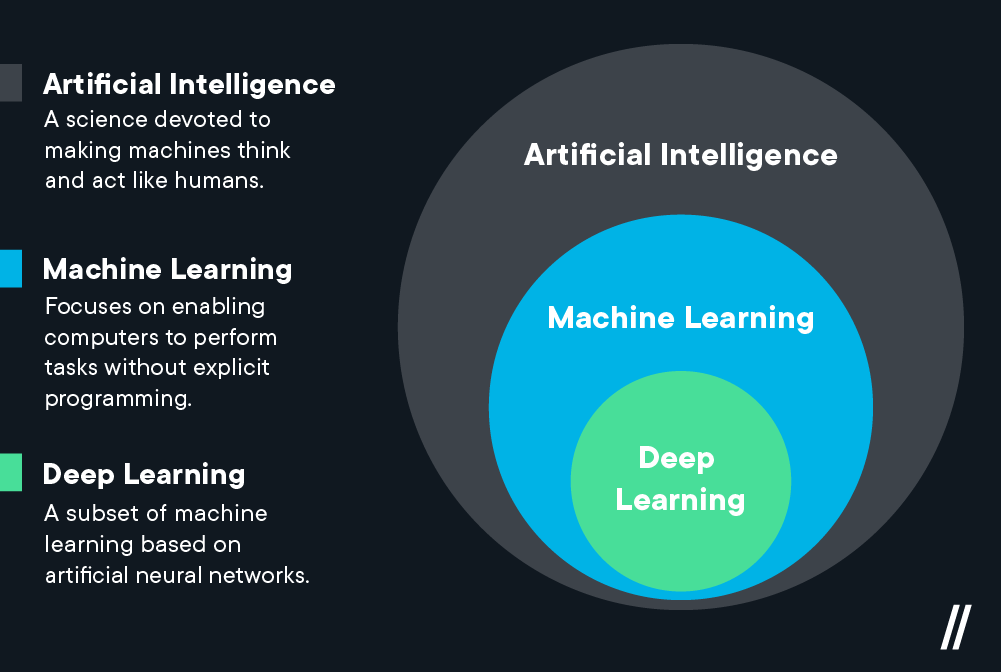
\includegraphics[width=0.75\linewidth]{Images/AI.png}
\end{figure}
\end{frame}

\begin{frame}{What is deep learning?}
\begin{minipage}{0.49\linewidth}
\begin{itemize}
\item Machine learning is a subset of statistics and computer science
\begin{itemize}
\item A set of rules (algorithm) or a model is trained, given inputs, to produce output (i.e., classification, regression) \item meaningfully transform data to learn useful representations
\end{itemize}
\item Deep learning is a subset of machine learning layered or hierarchical or multistage way to learn data representations (features)
\end{itemize}
\end{minipage}
\begin{minipage}{0.49\linewidth}
\begin{figure}
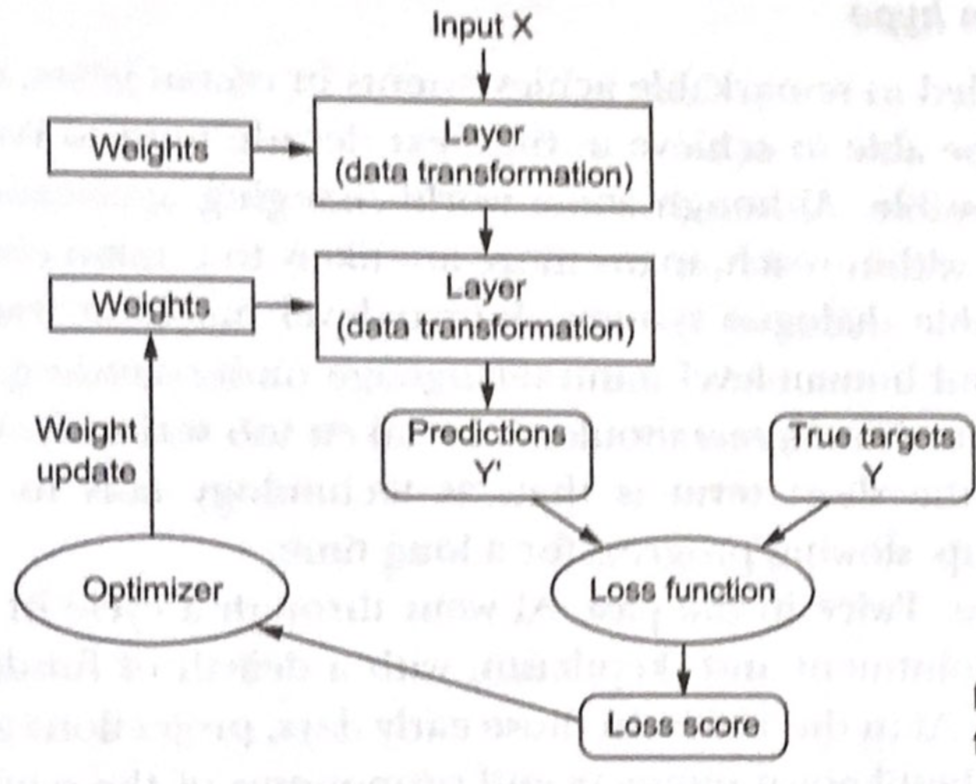
\includegraphics[width=\linewidth]{Images/DL.png}
\end{figure}
From Chollet and Allaire (2018)
\end{minipage}
\end{frame}
\subsection{Statistics vs deep learning}
\begin{frame}{Deep learning vs Statistics}
\begin{itemize}
\item Deep learning is tasked with estimating some quantity related to an output $\mathbf{Y}$, using inputs $\mathbf{X}$
\item We can think of this as making inference about some parameter $\hat{\mathbf{Y}}$, conditional on $\mathbf{X}$, by estimating some function $f:\mathbf{X}\rightarrow \hat{\mathbf{Y}}$ - this is just regression
\item Specification of $\hat{\mathbf{Y}}$ is done via some loss function and determines the type of problem we are dealing with
\begin{itemize}
\item For classification (logistic/multinomial regression), $\hat{\mathbf{Y}}$ may be a label or class probability
\item For prediction (mean regression), $\hat{\mathbf{Y}}$ is $\mathbf{E}[\mathbf{Y}|\mathbf{X}]$ 
\end{itemize}
\item The main difference between statistical, and deep, learning is the complexity of $f$. Statistics wants $f$ simple and easily interpretable, e.g, linear or additive, for explainability; DL wants the most complex $f$ that best optimises the loss
\end{itemize}

\end{frame}
\begin{frame}{A simple example: non-linear Gaussian regression}
\begin{itemize}
\item Consider a standard statistical problem: non-linear normal regression
\vfill
\item We will see that largely the \textbf{same methodology} is used to fit such models in statistics as in deep learning.

\item Say we want to fit a parametric model to these data:
\end{itemize}
\begin{figure}
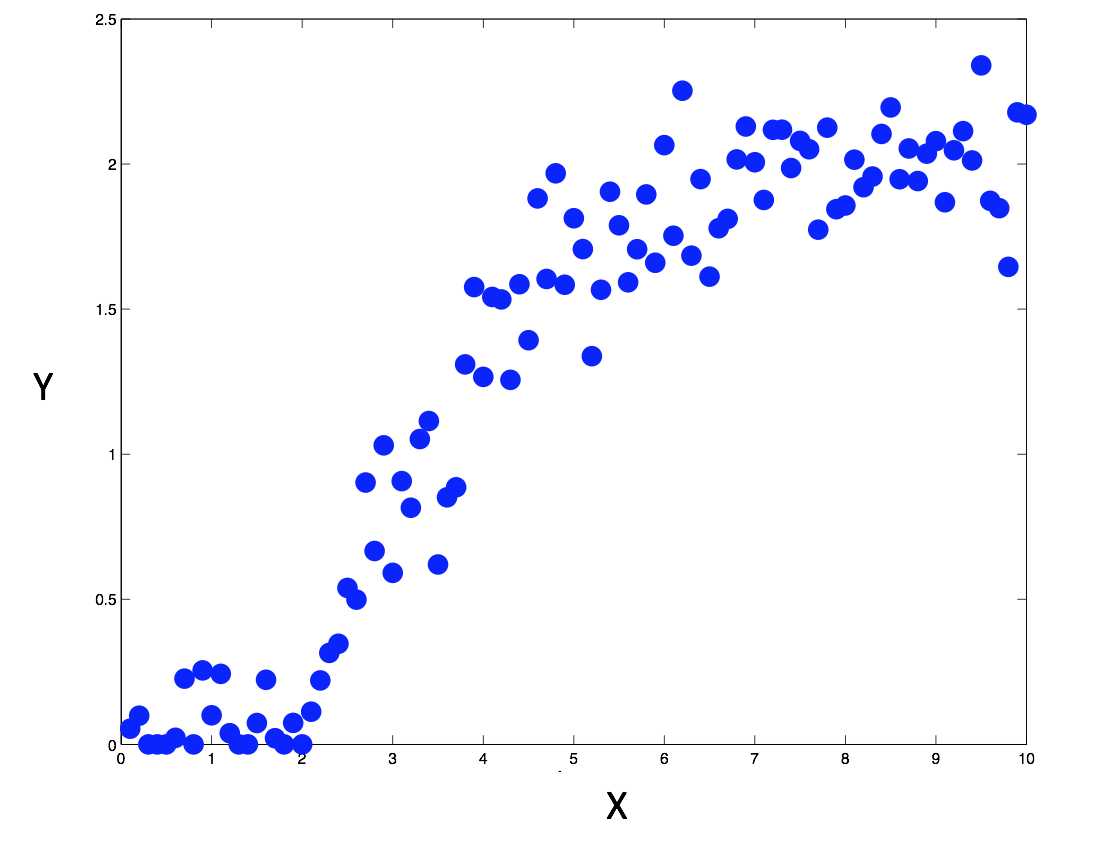
\includegraphics[width=0.6\linewidth]{Images/NL_reg.png}
\end{figure}
\end{frame}
\begin{frame}{A simple example: non-linear Gaussian regression}
A standard expectation regression model is of the form

$$
Y_{i}=f\left(\mathbf{X}_{i} ; \boldsymbol{\theta}\right)+\eta_{i}, \quad i=1, \ldots, n
$$

where $f\left(\mathbf{X}_{i} ; \boldsymbol{\theta}\right)$ is a \textbf{non-linear parametric function} such that $\mathrm{E}\left(Y_{i}|\mathbf{X}_i=\mathbf{x}_i\right)=f\left(\mathbf{x}_{i} ; \boldsymbol{\theta}\right)$. The function $f$ could be, e.g., polynomial, exponential, etc.
\begin{itemize}
\item $\mathbf{x}_{i}$ is a $p \times 1$ vector of observed predictors

\item $\boldsymbol{\theta}$ is a $q \times 1$ vector of parameters.

\item $\eta_{i}$ are i.i.d white noise.
\end{itemize}
\end{frame}
\begin{frame}{Loss function}
To fit our model, we minimize some loss function $Q(\hat{\mathbf{Y}},\mathbf{Y})$, where $\hat{\mathbf{Y}}$ is some model output (here the conditional expectation, with $\hat{{Y}}_i=f(\mathbf{X}_i)$).


For expectation regression, we typically select \textbf{squared-error loss} (e.g., residual sums of squares)

$$
Q(f(\mathbf{x}) ; \mathbf{y} ; \boldsymbol{\theta})=\sum_{i=1}^{n}\left\{{y}_{i}-f\left(\mathbf{x}_{i} ; \boldsymbol{\theta}\right)\right\}^{2},
$$
and seek:
$$
\hat{\boldsymbol{\theta}}=\underset{\boldsymbol{\theta}}{\operatorname{argmin}}\{Q(f(\mathbf{x}) ; \mathbf{y} ; \boldsymbol{\theta})\}.
$$
Note that this is equivalent to fitting a conditional Gaussian dist. (with homogeneous s.d.) via MLE. We may choose different $Q$ depending on how $\hat{Y}$ relates to $Y$, e.g., classification, MAE, statistical parameters. 
\end{frame}

\begin{frame}{Estimation}
We estimate $\hat{\boldsymbol{\theta}}$ via \textbf{numerical minimisation} of $Q$ based on some iterative gradient-based algorithm of the form

$$
\hat{\boldsymbol{\theta}}^{(j+1)}=\hat{\boldsymbol{\theta}}^{(j)}-\epsilon_{j} \mathrm{~A}_{j} \frac{\partial Q\left(\hat{\boldsymbol{\theta}}^{(j)}\right)}{\partial \boldsymbol{\theta}}
$$

where
\begin{itemize}
\item $\mathrm{A}_{j}$ is some positive definite matrix,

\item $\frac{\partial Q\left(\hat{\boldsymbol{\theta}}^{(j)}\right)}{\partial \boldsymbol{\theta}}$ (i.e., $\left.\nabla_{\theta} Q\left(\hat{\boldsymbol{\theta}}^{(j)}\right)\right)$ is the gradient of the objective function $Q(\boldsymbol{\theta})$ evaluated at $\hat{\boldsymbol{\theta}}$,

\item $\epsilon_{j}$ is the ''learning rate''. 
\end{itemize}
\end{frame}

\begin{frame}{Optimisation}
$$
\hat{\boldsymbol{\theta}}^{(j+1)}=\hat{\boldsymbol{\theta}}^{(j)}-\epsilon_{j} \mathrm{~A}_{j} \frac{\partial Q\left(\hat{\boldsymbol{\theta}}^{(j)}\right)}{\partial \boldsymbol{\theta}},
$$
\begin{itemize}
\item \textbf{Gradient Descent}: $A_{j} \equiv I_{p}$
\item Gauss-Newton: $A_{j} \equiv\left[F\left(\hat{\boldsymbol{\theta}}^{(j)}\right)^{\prime} \mathrm{F}\left(\hat{\boldsymbol{\theta}}^{(j)}\right)\right]^{-1}$, where $F(\theta) \equiv\left[\frac{\partial f\left(x_{i} ; \theta\right)}{\partial \theta_{j}}\right]$, the $n \times p$ Jacobian matrix
\item Levenberg-Marquardt: $A_{j} \equiv\left[F\left(\hat{\boldsymbol{\theta}}^{(j)}\right)^{\prime} \mathrm{F}\left(\hat{\boldsymbol{\theta}}^{(j)}\right)+\tau \right]^{-1}$ (Ridge penalty; $L_{2}$ regularization)
\item Newton-Raphson: $\mathrm{A}_{j} \equiv\left[\frac{\partial^{2} Q\left(\hat{\boldsymbol{\theta}}^{(j)}\right)}{\partial \boldsymbol{\theta} \partial \boldsymbol{\theta}^{\prime}}\right]^{-1}($ the $p \times p$ Hessian matrix)
\end{itemize}
\end{frame}
\begin{frame}{Optimisation}
\begin{itemize}
\item In general, optimization in machine learning algorithms usually consider a loss function that consists of a sum or average over the \textbf{entire training data} (e.g., all $n$ observations).
\item If $n$ is large, computation of the gradient can be slow. In addition, there may be \textbf{redundant data} in the training sample.
\end{itemize}
\end{frame}
\begin{frame}{Optimisation: SGD}
\begin{itemize}
\item One way to mitigate the aforementioned issues is to consider minimizing the \textbf{expected loss}. Estimation of the expected loss can be achieved by averaging the loss over small samples (\textbf{batches} or \textbf{minibatches}) of the training data (assuming the inputs $x_{i}$ are independently drawn from the same underlying distribution; not always reliable).
\item We refer to this as \textbf{stochastic} gradient descent, as the expectation of the gradient is estimated by \textbf{randomly} sampling a small number of samples of the training set and taking the average- this turns out to be a very effective solution to this problem.
\item Typically, smaller batch sizes offer more regularization and more flexibility (generalization) outside the training sample.
\end{itemize}
\end{frame}
\begin{frame}{SGD algorithm}
\textit{Basic Stochastic Gradient Descent} (SGD) Algorithm (Goodfellow et al. 2016, Chap. 8)

\textbf{Require}: Learning rate $\epsilon$\\
\textbf{Require}: Initial parameters $\boldsymbol{\theta}^{(j)}$\\
\;\;\;\;\textbf{while} Stopping criterion not met \textbf{do}\\
\;\;\;\;\;\;Sample a minibatch of $m$ inputs $\left\{\mathbf{x}_{1}, \ldots, \mathbf{x}_{m}\right\}$\\
\;\;\;\;\;\;\;\;and targets $\left\{\mathbf{y}_{1}, \ldots, \mathbf{y}_{m}\right\}$

\;\;\;\;\;\;Set $g=0$

\;\;\;\;\;\;\textbf{for} $i=1$ to $m$ \textbf{do}

\;\;\;\;\;\;\;\;Compute gradient estimate: $g \leftarrow g+\frac{1}{m} \nabla_{\boldsymbol{\theta}} Q\left(f\left(\mathbf{x}_{i} ; \boldsymbol{\theta}\right), \mathbf{y}_{i}\right)$

\;\;\;\;\;\;\textbf{end for}

\;\;\;\;\;\;Apply update: $\boldsymbol{\theta}^{(j+1)} \leftarrow \boldsymbol{\theta}^{(j)}-\epsilon \mathrm{g}$

\;\;\;\;\textbf{end while}
\end{frame}

\begin{frame}{SGD (cont.)}
\begin{itemize}
\item The learning rates are \textbf{quite important}. Large rates will cause the optimization to \textcolor{red}{diverge}; small rates may cause \textcolor{red}{convergence to local minima}. Algorithms exist for adaptive tuning of $\boldsymbol{\epsilon}$, most notably RMSprop\footnote{Unpublished Coursera course by Geoff Hinton \url{https://www.cs.toronto.edu/~tijmen/csc321/slides/lecture_slides_lec6.pdf}} and ADAM\footnote{\url{https://arxiv.org/abs/1412.6980} with over 111000 citations!}.
\item We may sometimes want to regularise the parameters in our model. This can be done by adding $L_2$ (ridge) or $L_1$ (lasso) penalties to the loss!
\item The framework is exactly the same for Deep learning, except now $f(\mathbf{X}_i; \boldsymbol{\theta})$ is a multi-layered neural network!
\end{itemize} 
\end{frame}
\subsection{Basics of neural networks}

\begin{frame}{Basics of neural networks}
\begin{minipage}{0.70\linewidth}
\begin{itemize}
\item A neural network is an algorithm designed to mimic the \textbf{human brain}.
\item It can be constructed as a \textbf{directed graph} with a single input and a single output, with a dense network of \textbf{interconnected nodes} in-between
\item Data is input into the graph and information is extracted at each node, a.k.a \textbf{perceptron}. An output is provided at the end of the network.
\item Similarly brain activity occurs when a stimuli enters the system, information is based through the network via \textbf{neurons} that extra relevant information and this information passes to some area of the brain that forces a response (output)
\end{itemize}
\end{minipage}
\begin{minipage}{0.29\linewidth}
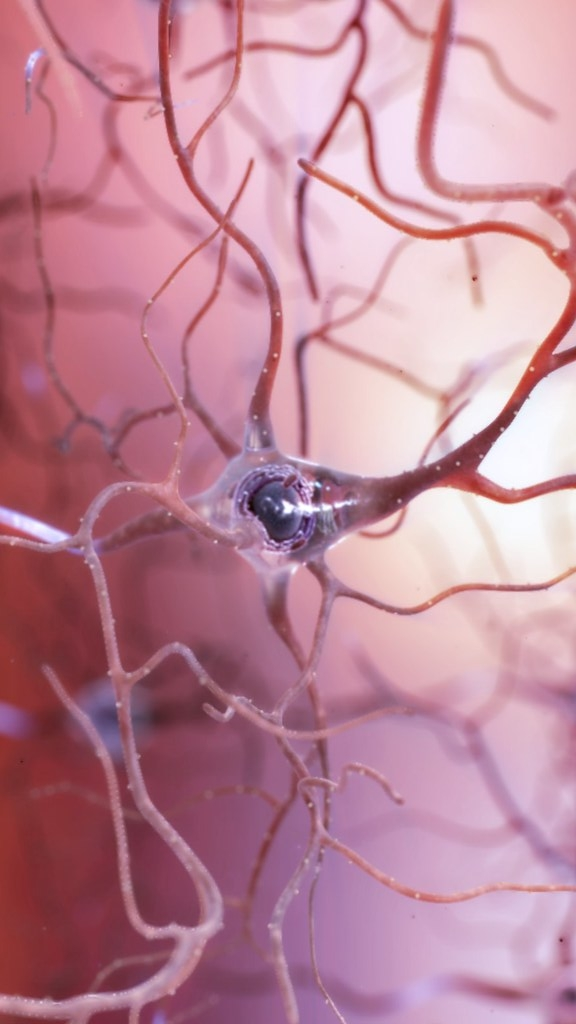
\includegraphics[width=0.9\textwidth]{Images/neuron.jpg}
\end{minipage}
\end{frame}
\begin{frame}{Basics of neural networks (cont.)}
 Nodes in a neural network are arranged in layers:
\begin{itemize}
\item A single node may be connected to several nodes in the layer above, from which it \textbf{receives information}, and to the layer below, which it \textbf{feeds information}
\item Most neural networks are \textbf{``feed forward''} - information is passed forward, layer-to-layer, in one direction only (but we also consider RNN)
\item Different information (features) is extracted at each layer in a \textbf{hierarchical} fashion, i.e., the most important aspects first
\item The ``deep'' in deep learning refers to the depth of layers in a neural network as well as its hierarchical nature
\item Each layer can be considered as a non-linear regression of inputs from the previous layer; a neural network is simply a composition of non-linear regressions
\end{itemize}
\end{frame}
\begin{frame}{General structure}
\begin{itemize}
\item A \textbf{single input layer}. Each input would be a single predictor variable in the form of a scalar value, a sequence or an image (or even a sequence of images!).
\item \textbf{A single output layer}. For prediction or classification problems, we would have a single node here. 
\item A collection of \textbf{hidden layers} of variable \textbf{widths}. Preferably more than one!
\item Calculations are completed at each node in the hidden layer. These are parameterised by \textbf{weights and biases}.
\item In Keras, calculations within a layer are of a certain ``type''. We will consider standard (\textbf{vanilla}), convolution and recurrent layers.
\end{itemize}
We refer to the structure of a neural network as its \textbf{architecture}.
\end{frame}
\begin{frame}{Single layer neural network}
\begin{itemize}
\item Let's first consider a simple feed-forward NN with a single hidden layer, a.k.a, a \textbf{single layer perceptron}
\item Takes input $p$-dimensional input $\mathbf{x}$, $k$-dimensional output $\hat{\mathbf{y}}$ (although $k=1$ for most problems) and single hidden layer $\mathbf{z}$ (hence ``\textbf{shallow}'')
\end{itemize}
\begin{figure}
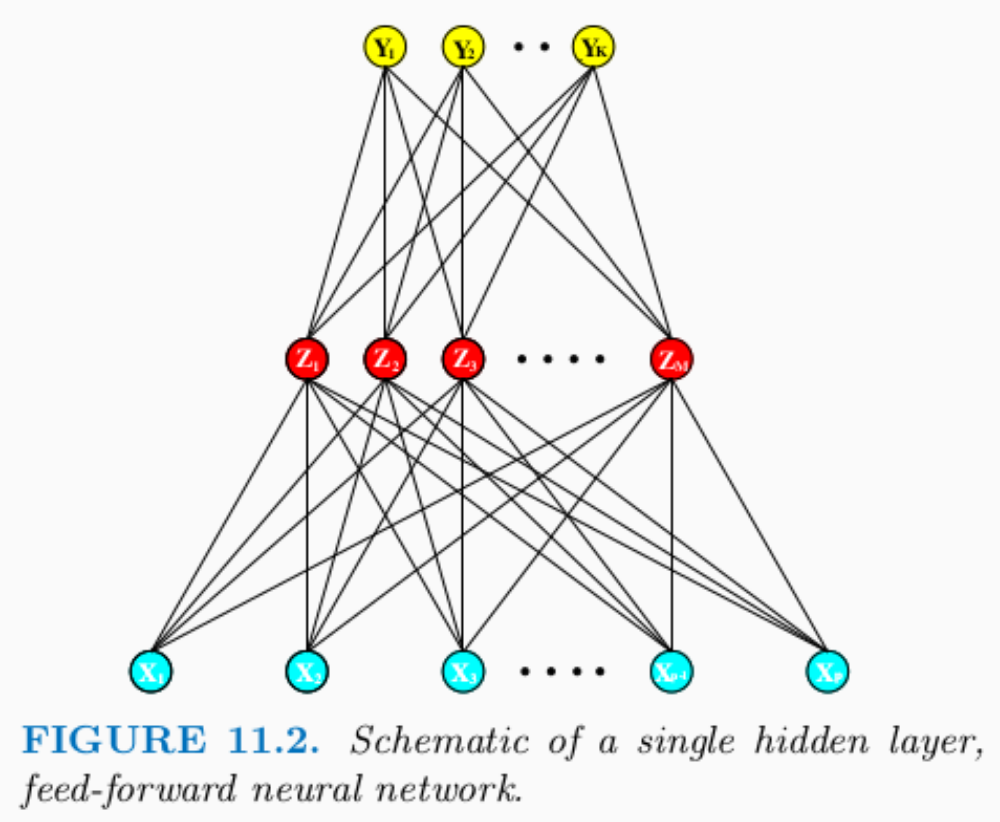
\includegraphics[width=0.48\linewidth]{Images/singleNN.png}
\end{figure}
[Hastie et al. 2009, Fig. 11.2.]
\end{frame}


\begin{frame}{Single layer FNN: hidden layer}
A hidden layer in a perceptron is implemented using  $\texttt{layer\_dense}$ in $\texttt{Keras}$.\\
\textbf{Hidden Layer}:
$$
z_{j}=g\left(\alpha_{j 0}+\sum_{i=1}^{p} \alpha_{j i} x_{i}\right), \quad j=1, \ldots, J,
$$

where $z_{j}$ is the hidden variable, $\alpha_{j 0}\in\mathbb{R}$ is bias, $\left\{\alpha_{j i}\right\}\in\mathbb{R}$ are the weight parameters, and $g(\cdot)$ is the activation function.\\
It simplifies notation to assume $x_{0}=1$ and then

$$
z_{j}=g\left(\sum_{i=0}^{p} \alpha_{j i} x_{i}\right), \quad j=1, \ldots, J
$$
\end{frame}

\begin{frame}{Activation functions\footnote{\url{https://en.wikipedia.org/wiki/Activation_function}}}
The activation function defines the \textbf{output of the node}. There's a range of different functions that you can use (see \url{https://keras.rstudio.com/reference/activation_relu.html}), but typically they must satisfy two properties:  
\begin{itemize}
\item \textbf{Nonlinear}! If all nodes had linear activation, this would just be a linear regression model. A two-layered NN with non-linear activations is a \textbf{universal function approximator}.
\item \textbf{``Continuously'' differentiable}. Needed for gradient-based optimisation.
\end{itemize}
You can think of the activation function as an analogue to the link function in regression. 
\end{frame}
\begin{frame}{ReLu activation}
An activation function that's popularly applied is the \textbf{rectified linear unit}:
\begin{itemize}
\item Older neural networks relied on sigmoid or $\tanh$ activation functions
\item These suffered from the \textit{vanishing gradient problem}\footnote{The networks we will be considering will not be overly deep, so this problem does not occur. For details, see \url{https://machinelearningmastery.com/rectified-linear-activation-function-for-deep-learning-neural-networks/}}, which made it \textcolor{red}{difficult to efficiently train deep networks}
\item The ReLU replaced these. It has the form $g(x)=\max\{x,0\}$.
\end{itemize}
\begin{minipage}{0.49\linewidth}
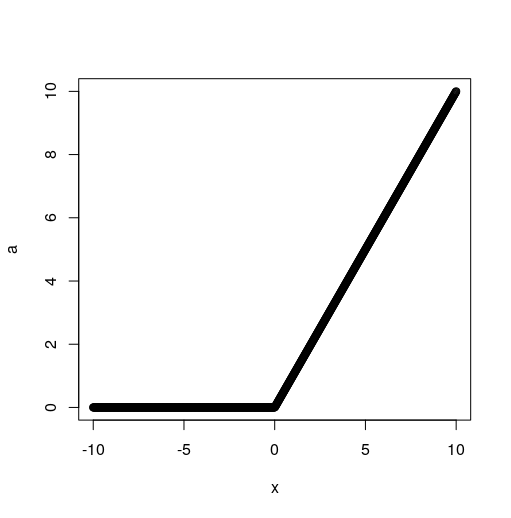
\includegraphics[width=0.5\textwidth]{Images/ReLu.png}
\end{minipage}
\begin{minipage}{0.49\linewidth}
\begin{itemize}
\item The neuron ``activates'' only if \textbf{enough information passes through} (think pain receptors)
\item One drawback: \textcolor{red}{not differentiable at zero}
\end{itemize}
\end{minipage}
\end{frame}

\begin{frame}{Single layer FNN: output layer}
\textbf{Output Layer}:
$$
\hat{y}_{k}=h\left(\beta_{k 0}+\sum_{j=1}^{J} \beta_{k j} z_{j}\right), \quad k=1, \ldots, K,
$$
where $\hat{y}_{k}$ is the output variable and $h(\cdot)$ is another activation function, which must be carefully selected to enforce range constraints on the output $\hat{\mathbf{y}}$. We may take the identity function for mean/median regression or a sigmoid or softmax function for classification.\\

As with the hidden layer, we can write

$$
\hat{y}_{k}=h\left(\sum_{j=0}^{J} \beta_{k j} z_{j}\right), \quad k=1, \ldots, K.
$$
\end{frame}
\begin{frame}{Singe layer FNN (cont.)}
In summary, the single layer feed-forward NN can be written:

$$
\hat{y}_{k}(\mathrm{x} ; \boldsymbol{\beta}, \boldsymbol{\alpha})=h\left(\sum_{j=0}^{J} \beta_{k j} g\left(\sum_{i=0}^{p} \alpha_{j i} x_{i}\right)\right).
$$
As with traditional statistical regression, we estimate the parameters (or ''train the network'') by choosing an objective function $Q(\hat{\mathbf{y}},\mathbf{y}; \boldsymbol{\alpha}, \boldsymbol{\beta})$ and then use stochastic gradient descent to obtain parameter estimates of the weight/bias vectors, $\boldsymbol{\alpha}$ and $\boldsymbol{\beta}$.

Note that this formulation illustrates that an NN is just a \textbf{composition of non-linear activations of convex sums}.
\end{frame}
\begin{frame}{Loss functions}
 Whilst the NN architecture can be standard for any task, the loss function $Q$ must be \textbf{very specific}! Examples include:
\begin{itemize}
\item MSE: $(1/n)\sum^n_{l=1}(y_l-\hat{y}_l)^2$ (mean prediction)
\item MAE: $(1/n)\sum^n_{l=1}|y_l-\hat{y}_l|$ (median prediction)
\item binary cross-entropy (if $\hat{y}_l\in(0,1)$ and $y_l=0$ or $1$): $-(1/n)\sum^n_{l=1}(y_l\log\hat{y}_l+(1-y_l)\log(1-\hat{y}_l))$. Two-class classification, but can be extended to more than two classes.
\item \textbf{negative log-likelihood}, where $\hat{y}$ are model parameters
\end{itemize}
\end{frame}

\subsection{Backpropogation}
\begin{frame}{Backpropagation}
In order to use SGD, we require the negative log-likelihood of $Q$ w.r.t the weight/biases. This may seem like a fairly daunting task, particularly if we have many weights or additional layers. However,  the neural net community uses an algorithm called ''\textbf{backpropagation}'' to evaluate the gradients very quickly; this is nothing more than iterative application of the chain rule, which is particularity easy due to the hierarchical nature of the model.

$$
\begin{aligned}
\frac{\partial Q}{\partial \alpha_{j i}} & =\frac{\partial Q}{\partial \hat{y}_{k}} \frac{\partial \hat{y}_{k}}{\partial z_{j}} \frac{\partial z_{j}}{\partial \alpha_{j i}}, \quad j=1, \ldots, J ; i=0, \ldots, p \\
\frac{\partial Q}{\partial \beta_{k j}} & =\frac{\partial Q}{\partial \hat{y}_{k}} \frac{\partial \hat{y}_{k}}{\partial \beta_{k j}}, \quad k=1, \ldots, K ; j=0, \ldots, J.
\end{aligned}
$$
\end{frame}
\begin{frame}{Illustrating back propagation}
Let's take a simple illustration. Consider a fairly simple case of nonlinear regression with a single output, $h(\cdot)$ the identity function, $g(\cdot)$ the sigmoid function, and squared error loss.
\begin{align}
\hat{y} & =\sum_{j=0}^{J} \beta_{j} z_{j}, \\
z_{j} & =g\left(\sum_{i=0}^{p} \alpha_{j i} x_{i}\right).
\end{align}


Squared-error objective function:

$$
Q(\hat{{y}},{y}; \boldsymbol{\alpha}, \boldsymbol{\beta})=\frac{1}{2} \left({y}-\hat{y}\right)^{2}.
$$
\end{frame}
\begin{frame}{Illustrating back propagation}
The gradients are given by:
\begin{align}
 \frac{\partial Q}{\partial \beta_{k j}}&=\frac{\partial Q}{\partial \hat{y}_{k}} \frac{\partial \hat{y}_{k}}{\partial \beta_{k j}}=-\left(-\hat{y}\right) z_{j} \\
\frac{\partial Q}{\partial \alpha_{j i}} & =\frac{\partial Q}{\partial \hat{y}_{k}} \frac{\partial \hat{y}_{k}}{\partial z_{j}} \frac{\partial z_{j}}{\partial \alpha_{j i}}\nonumber \\
& =\left\{-\left(y-\hat{y}\right)\right\}\left\{\beta_{j}\right\}\left\{z_{j}\left(1-z_{j}\right) x_{i}\right\}
\end{align}
Note: $\partial g(a b) / \partial a=g(a)(1-g(a)) b$ when $g(\cdot)$ is a sigmoidal function.\\
The gradients extend \textbf{as expected} when more hidden layers are introduced, e.g., a two layered model will have an extra set of weights, and three equalities with a product of two, three and four terms.
\end{frame}
\begin{frame}{Backpropogation (cont.)}
The gradient vectors fed in SGD and \textbf{updates are done in a two-pass algorithm}.
\begin{itemize}
\item In the \textbf{forward pass}, the current weights values are fixed and $z_{j}$ and $\hat{y}$ are calculated using $(1)$ and $(2)$
\item In the \textbf{backward pass}, the gradients are then calculated from (3) and (4); then, the parameters are updated using the SGD updates shown earlier.
\end{itemize}
An important feature of backpropagation algorithms is that each hidden unit passes and receives information only to and from units that share a connection - i.e., it is a ''local'' algorithm. This facilitates computation in a parallel computing environment, which is important for large datasets.
\end{frame}

\begin{frame}{Automatic differentiation}
\begin{itemize}
\item Note that you \textbf{never have to calculate derivatives} to implement backpropagation.

\item Deep learning software packages all include some form of automatic differentiation that can symbolically/algorithmically work out the derivatives for you. Derivatives for standard loss and activations will be hardcoded explicitly.

\item  As long as we construct \textbf{differentiable loss and activation functions}, backpropagation can be performed very efficiently!\linebreak
When writing custom functions for \texttt{Keras}, we \textbf{must use the} \texttt{tensorflow} or  \texttt{Keras} backend functions; these have \textbf{known derivatives} that \texttt{tensorflow} can easily call.
\end{itemize}
\end{frame}
\begin{frame}{Deep neural networks}
Putting the \textbf{deep} in \textbf{deep} learning:
\begin{itemize}
\item Deep neural networks generalise the previously seen single layer network to \textbf{multiple layers}
\item The outputs from one layer become the input of the next. We consider the number of units in each layer as the \textbf{width} and the number of layers as the \textbf{depth} of the network. Having both width and depth provides a \textbf{very flexible learning environment}.
\item The biggest challenge with implementing deep models is that they are often \textbf{severely over-parameterized} and easily over-fit
\item With many parameters, we may also experience \textbf{vanishing} or \textbf{exploding} gradients; theses issues can be mitigated with data pre-processing and weight initialisation
\end{itemize}
\end{frame}

\begin{frame}{Typical structure\footnote{Copyright belongs to \url{https://www.ibm.com/cloud/blog/ai-vs-machine-learning-vs-deep-learning-vs-neural-networks}}}
\begin{figure}
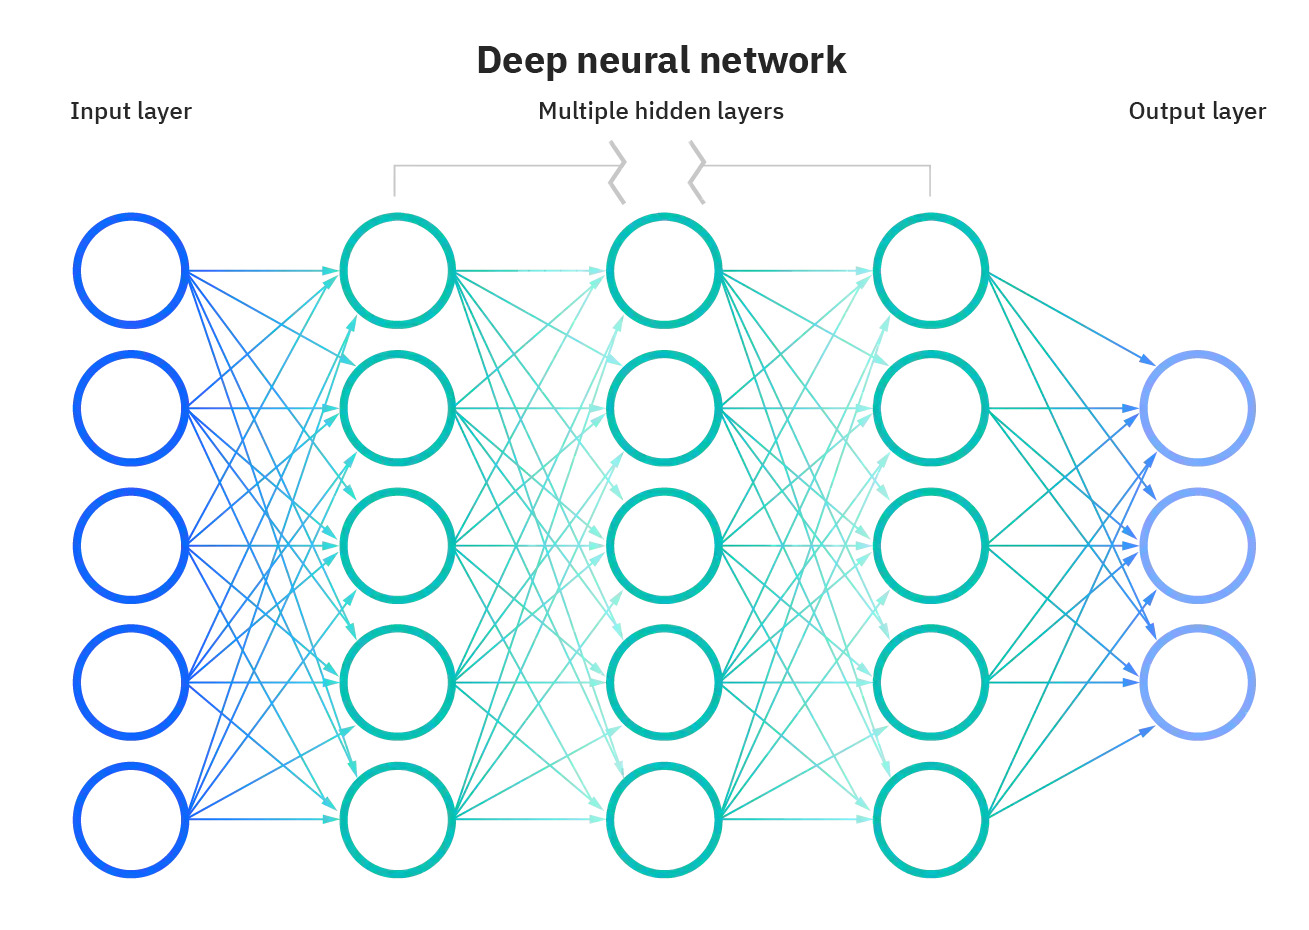
\includegraphics[width=0.7\textwidth]{Images/nn.jpg}
\end{figure}
\end{frame}
\begin{frame}{Deep FFNN: 2-layered example}
An MLP with two hidden layers and one output can be written:
$$
\begin{gathered}
z_{1 j}=g_1\left(\sum_{i=0}^{p} \alpha_{1 j i} x_{i}\right), \quad j=1, \ldots, J_{1}, \\
z_{2 j^{\prime}}=g_2\left(\sum_{j=1}^{J_{1}} \alpha_{2 j^{\prime} j} z_{1 j}\right), \quad j^{\prime}=1, \ldots, J_{2}, \\
\hat{y}=h\left(\sum_{j^{\prime}=0}^{J_{2}} \beta_{j^{\prime}} z_{2 j^{\prime}}\right).
\end{gathered}
$$
Training follows with backpropagation in the same way as for the one-hidden layer model; the gradient vectors generalise as expected.
\end{frame}

\section{Implementation and regularisation}
\begin{frame}
\begin{center}
\item Some things to consider when implementing large models to avoid numerical instabilities in training or overfitting
\end{center}
\end{frame}
\begin{frame}{Training/validation/testing}
Due to their \textcolor{red}{large number of parameters}, neural networks are \textcolor{red}{prone to overfitting}. It's necessary to use \textbf{validation/testing} to assess any overfitting.
\begin{itemize}
\item First, we subset the data into training, validation and testing. Opinions differ, but the standard is $80/10/10$
\item Each set has a different purpose:
\begin{itemize}
\item The model is \textbf{trained} on the training data. This is used to optimise the weights, biases and other hyper-parameters
\item We then \textbf{validate} the model by getting predictions for the validation set and evaluating validation loss. This will give us some insight as to whether or not overfitting is occurring. Typically the validation loss is used for model selection
\item To get a truly unbiased evaluation of the model fit and to compare amongst different models, we should \textbf{test} the model on  previously unseen data
\end{itemize}
\end{itemize}
\end{frame}

\begin{frame}{Mitigation}
\begin{itemize}
\item Some literature uses \textbf{test} and \textbf{validation} interchangeably, e.g., in cross-validation, the validation (hold-out) set is actually a test set because the model never sees it for training
\item Overfitting in neural networks is \textbf{inevitable} if a network is trained \textbf{indefinitely}. 
\item However, you can mitigate the risk of fitting using forms of regularisation. 
\end{itemize}
\end{frame}
\begin{frame}{Initialisation}
Although the backpropagation algorithm is simple, the challenge is to implement it in a way that is practical and generalizable, particularly for large networks. Some considerations should be taken when initialising a model.\\

\textbf{Normalisation/standardisation}: 
\begin{itemize}
\item The inputs into a neural network should be standardised so that features have the same scale. Common approaches include: subtracting the mean and dividing by the standard deviation; mapping all features to $[0,1]$ by subtracting the max and dividing by the range. Note that both the training and test/validation data must be standardised in the exact same manner
\item Batch normalisation: outputs of a hidden layer within a neural network are centered and scaled using the $\texttt{layer\_batch\_normalization}$ in $\texttt{Keras}$
\end{itemize}
\end{frame}
\begin{frame}{Initialisation}
\textbf{Weight initialization:}
Given the highly nonlinear nature of neural models, they can be very sensitive to the initial parameter values. Two general heuristic ''principles'' to consider:
\begin{itemize}
\item choose initial weights such that each hidden variable is operating in the linear range of its activation function, i.e., not so large or small that the derivative is initialised at zero; as this depends on both the weights and the inputs, this is why we standardize the inputs
\item choose initial weights randomly (hidden units are interchangeable; one needs them to find different features, so it is important that they not have the same weights) (default in Keras)
\end{itemize}
Exception: pre-training, \textbf{pathological likelihoods}
\end{frame}
\begin{frame}{Regularisation}
In order to mitigate overfitting, consider the following regularisation techniques:\\
\textbf{Penalties:}
The most common is to consider an $L_{2}$ (ridge) penalty to the objective function of the form, e.g., in our simple example, $\lambda\left(\sum_{j i} \alpha_{j i}^{2}+\sum_{k j} \beta_{k j}^{2}\right)$, where $\lambda \geq 0$ is some tuning parameter. This has the effect of adding terms $2 \lambda \beta_{k j}$ and $2 \lambda \alpha_{j i}$ to the gradient expressions, and shrinks the weights to zero.\\

Can use $L_{1}$ (Lasso) as an alternative - this provides full weight elimination, in which small parameters are set to zero - or a mix of the two.
\end{frame}
\begin{frame}{Regularisation}
\textbf{Dropout:}
An alterative form of regularisation is \textbf{dropout}.\\
The idea is straightforward: randomly omit a certain (relatively small) percentage (say, $\gamma$ ) of the hidden units in each hidden layer for each minibatch of samples during the backpropagation training.\\
This helps to \textbf{break up the dependence} in the hidden units and prevents overfitting. It is easy to implement dropout - just set the activation to 0 (no information propagates through that unit, and so the algorithm doesn't have to be changed in any other way).\\

Implemented via $\texttt{layer\_dropout}$ in $\texttt{Keras}$.
\end{frame}
\begin{frame}{Regularisation}
\textbf{Early stopping:}\\
\textcolor{blue}{Rarely does the best generalization of a deep model occur at the local minimum obtained by the gradient descent algorithm}. Thus, an important form of regularization that facilitates generalization is called early stopping, which simply means one stops the gradient descent algorithm before it has fully converged to a minima of the loss.\\
Neural networks are trained for a pre-fixed number of iterations (\textbf{epochs}). At which epoch to stop training can be inuited as an extra hyperparameter that must be chosen \textbf{via validation} or by trial-and-error. This is the easiest type of regularisation one can do as it doesn't require any change to the basic algorithm and can be used (and typically is) with other forms of regularization (e.g., weight decay, dropout, etc.).
\end{frame}
\begin{frame}{Regularisation}
\textbf{Weight sharing and parsimonity:}\\
\textcolor{blue}{Reduce the number of trainable weights!}\\
In some types of deep models, it makes sense that weights should be similar (e.g., imagine weights connected to components of an image or in a sequence of words). One can force these weights to be identical, or can add a penalty term that favours them being similar (we will see such an example with convolutional NNs).\\
Using a neural network that's adapted to your task may provide you with a model that's easier and faster to train, with less estimable parameters.
\end{frame}

\begin{frame}{Regularisation}
\textbf{Data augmentation}\\
Neural networks typically require a lot of data to train! Overfitting is more prevalent with fewer training samples from which to learn, which prevents the model from being able to generalize to new data.\\

For some models (e.g., CNNs), it is possible to use data augmentation to \textbf{generate more training data from existing training samples} by transforming inputs to produce new input samples that are similar, but different, to the training data, e.g., rotating images. 
\end{frame}

\begin{frame}{Regularisation}
\textbf{Pre-training}\\
We can often save time when training networks by using the parameters from a pre-trained model as initial values in backpropogation. This is particularly useful if you want:
\begin{itemize}
\item Repeated model fits, e.g., a \textbf{bootstrap analysis}
\item \textbf{To train a very complex model}. Very complicated models are commercially trained on massive datasets (e.g., ImageNet, which has 1000 \textbf{categories} and $1.4$ million images), with substantial computational resources. A user can take a pre-trained model and then re-train the model on their own data (potentially treating some hidden layers as fixed a priori)
\end{itemize}
\end{frame}

\begin{frame}{Hyper-parameters}
There are hyper-parameters we need to consider when building and training neural networks:\\
\textbf{Batch-size:}\\
As discussed, using batches of data in stochastic gradient descent is \textbf{computationally advantageous}. In deep learning, one divides the training samples by the batch size and cycles through all training data in a single \textbf{epoch}.\\
Smaller batch-size $\Rightarrow$ faster training, but more volatile\\
Larger batch-size $\Rightarrow$ slower training, but more regular convergence (particularly with \textbf{highly dependence inputs}!)\\
It may be preferable to have large gradient variance at the beginning of the optimization so the solution can jump out of local minima; hence we could also use a varying sample size across training.
\end{frame}

\begin{frame}{Hyper-parameters}
\textbf{Architecture:}\\
The number of layers and the number of hidden units in each layer are also hyper-parameters that need to be chosen. Other than the fact that we need enough hidden units to capture structure, and we don't want ''too many'' (to prevent overfitting), choosing the complexity isn't an exact art. This is very much the ''art'' of deep modelling.\\

In general, wide/shallow models are easier to overfit and narrow/deep models are easier to underfit. It is often recommended that the lower levels have more hidden units, but bottlenecks in networks can also be helpful.\\
We can choose the architecture through model \textbf{testing} (not validation!). I typically start with a standard architecture (across all projects) and then just iteratively test changes in complexity.
\end{frame}
\begin{frame}{Hyper-parameters}
\textbf{Others:}\\
\begin{itemize}
\item Learning rate decay in optimisers
\item Dropout rate
\item Smoothing penalty tuning parameters
\item Early-stopping
\end{itemize}
\end{frame}
\section{Convolutional neural networks}
\begin{frame}{Convolutional neural networks (CNNs)}
\begin{itemize}
\item One of the early success stories in multi-level neural networks occurred with so-called ``\textbf{convolutional neural networks} (CNNs)” applied to image classification (e.g., LeCun and colleagues in the 1990s).
\item CNNs are successful because the patterns they learn are \textbf{translation invariant} and they can learn \textbf{spatial hierarchies of patterns}. Whilst densely-connected networks learn global patterns in their input feature space, convolution layers learn local patterns.
\item Before we talk about convolutional networks, we review a bit about
convolution, especially as it applies to images.
\end{itemize}
\end{frame}
\begin{frame}
\begin{center}
\Huge Convolutional neural networks
\end{center}
\end{frame}
\begin{frame}{Convolution}
Basic Mathematical Definition:

$$
(f * g)(t)=\int_{\mathbb{R}^{d}} f(\tau) g(t-\tau) d \tau=\int_{\mathbb{R}^{d}} f(t-\tau) g(\tau) d \tau .
$$

Discrete convolution (e.g., $\mathrm{d}=2 \mathrm{dim}$ ) [in practice, these are finite sums]

$$
f[x, y] * g[x, y]=\sum_{i=-\infty}^{\infty} \sum_{j=-\infty}^{\infty} f[i, j] g[x-i, y-j]
$$

So, we can think of $f[]$ as a ''kernel'' weight function that is applied to elements of the spatial image $g[]$. We are familiar with this concept in terms of kernel smoothing; note that in kernel smoothing, the kernels must integrate to 1 (or sum, in the case of discrete data) - this is not the case for convolution - but, we sometimes still call them \textbf{kernels} or \textbf{filters}.
\end{frame}
\begin{frame}{Convolution: 1-d example}
\begin{figure}
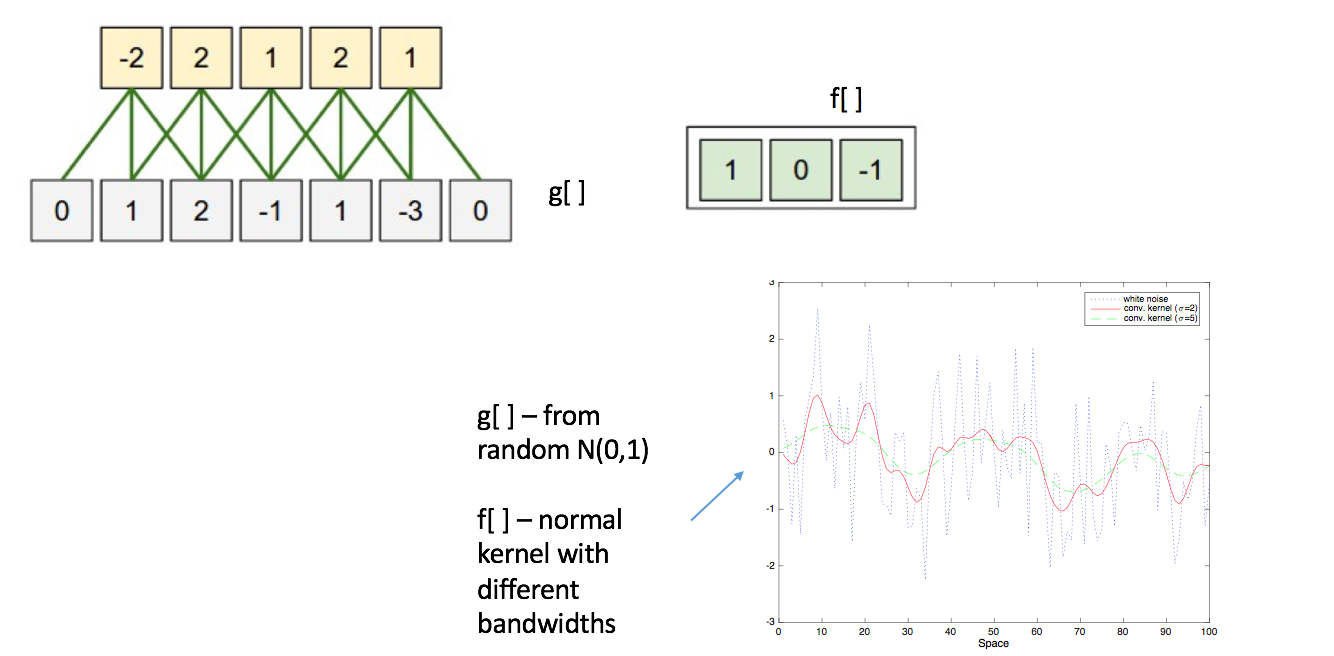
\includegraphics[width=\textwidth]{Images/1dconv.png}
\end{figure}
\centering \copyright C. K. Wikle and D. Pagendam
\end{frame}
\begin{frame}{Convolution: 2-d example}
\begin{figure}
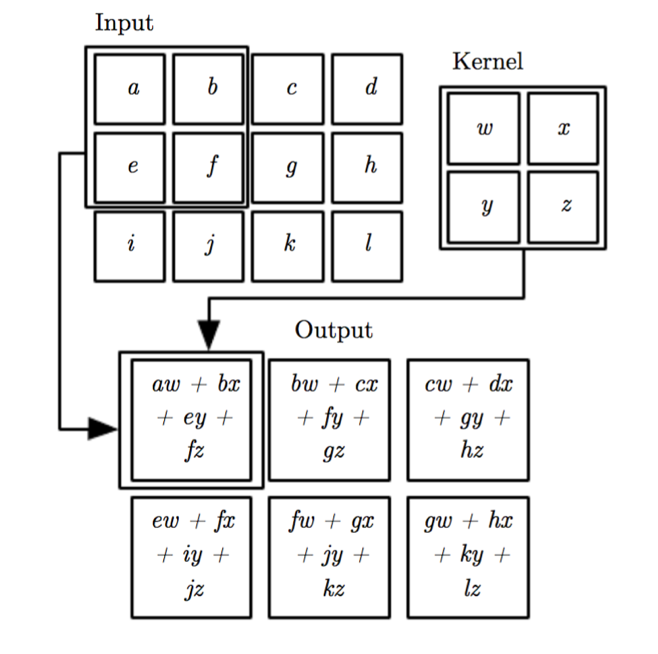
\includegraphics[width=0.45\linewidth]{Images/2dconv.png}
\end{figure}
\centering \copyright C. K. Wikle and D. Pagendam \\
Note the \textbf{edge effect} - the convolved image is smaller. This can be avoided by \textbf{padding} the original image with zeroes around the edges.
\end{frame}

\begin{frame}{Image convolutions\footnote{Following done using the $\texttt{OpenImageR}$ package}}
Different kernel weights extract different features from images.\\
\textbf{Consider this handsome fellow:}
\begin{figure}
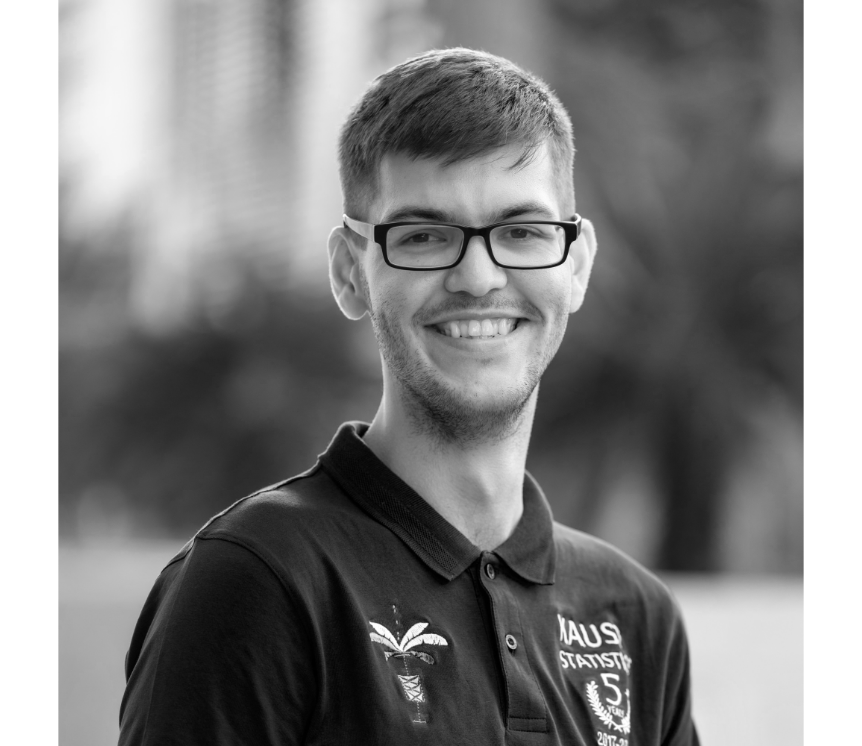
\includegraphics[width=0.45\linewidth]{Images/conv1.png}
\end{figure}
\end{frame}

\begin{frame}{Image convolutions}
What happens when we apply this first kernel?

\begin{minipage}{0.32\linewidth}
\begin{figure}
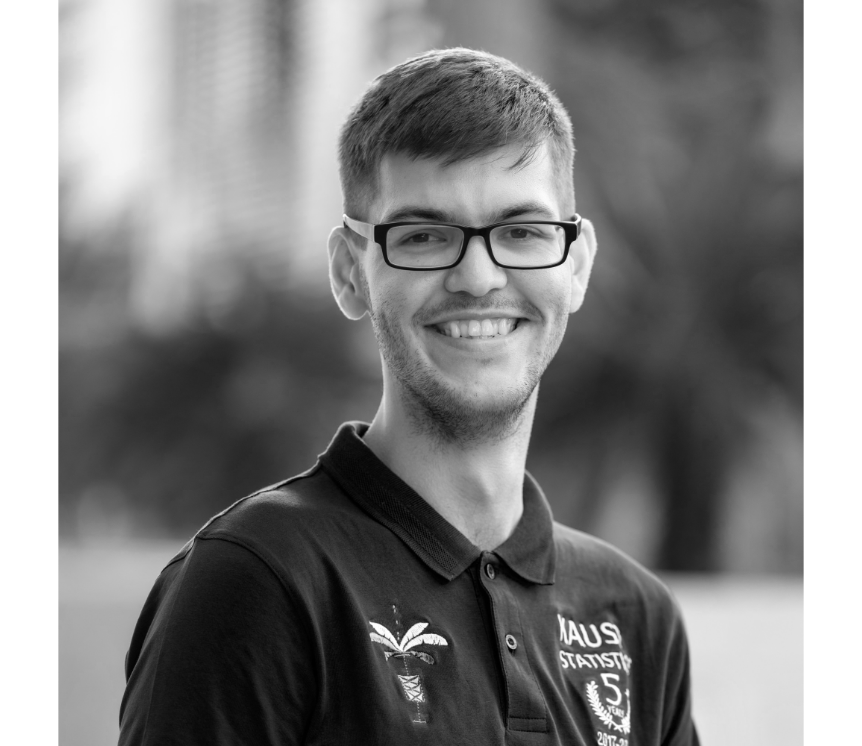
\includegraphics[width=\linewidth]{Images/conv1.png}
\end{figure}

\end{minipage}
\begin{minipage}{0.32\linewidth}
$ * \frac{1}{25}\begin{pmatrix}
1 & 1 & 1 & 1 &1 \\
1 & 1 & 1 & 1 &1 \\
1 & 1 & 1 & 1 &1 \\
1 & 1 & 1 & 1 &1 \\
1 & 1 & 1 & 1 &1 \\
\end{pmatrix} =$
\end{minipage}
\begin{minipage}{0.32\linewidth}
\begin{figure}
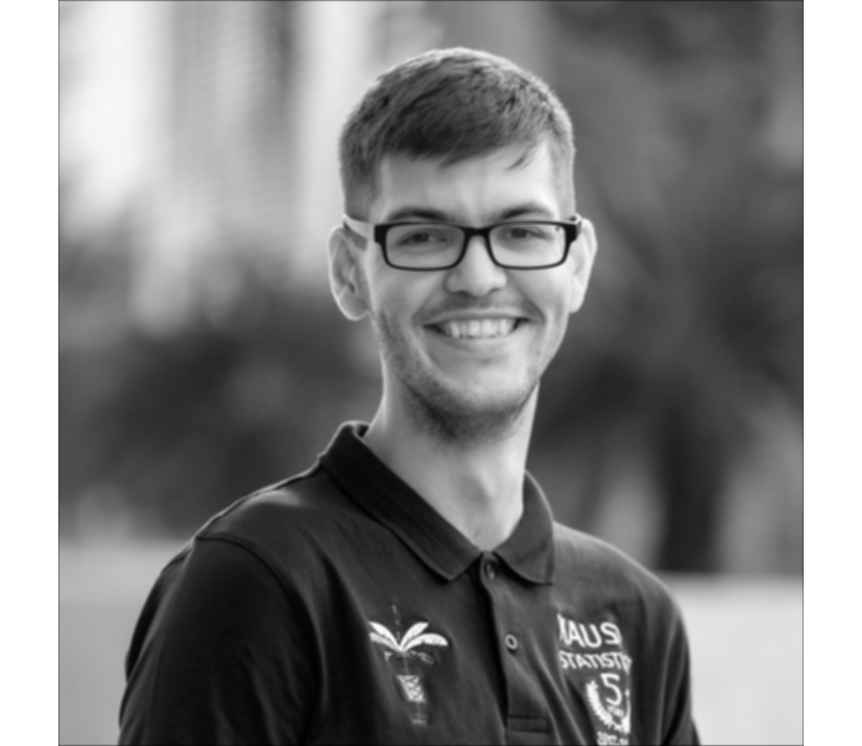
\includegraphics[width=\linewidth]{Images/conv2.png}
\end{figure}
\end{minipage}
\end{frame}

\begin{frame}{Image convolutions}
And this second one?

\begin{minipage}{0.32\linewidth}
\begin{figure}
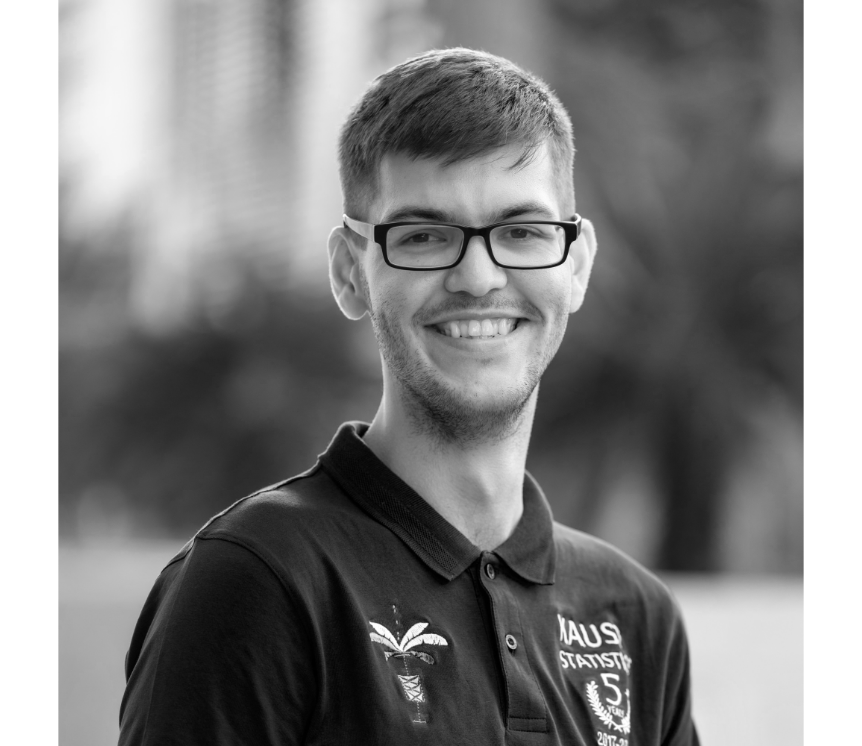
\includegraphics[width=\linewidth]{Images/conv1.png}
\end{figure}

\end{minipage}
\begin{minipage}{0.32\linewidth}
$ * \begin{pmatrix}
0& 0 & 0 \\
1& 0 & 0 \\
0& 0 & 0 \\
\end{pmatrix} =$
\end{minipage}
\begin{minipage}{0.32\linewidth}
\begin{figure}
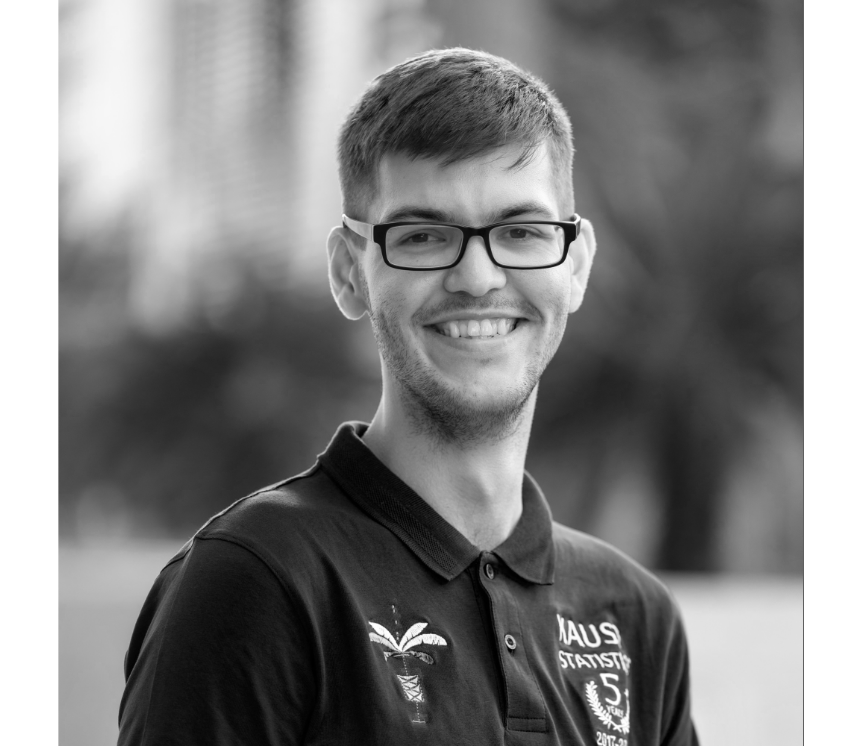
\includegraphics[width=\linewidth]{Images/conv3.png}
\end{figure}
\end{minipage}
\end{frame}

\begin{frame}{Image convolutions}
If we subtract the two images, we see that the kernel shifts the image 1 pixel to the left. 

\begin{figure}
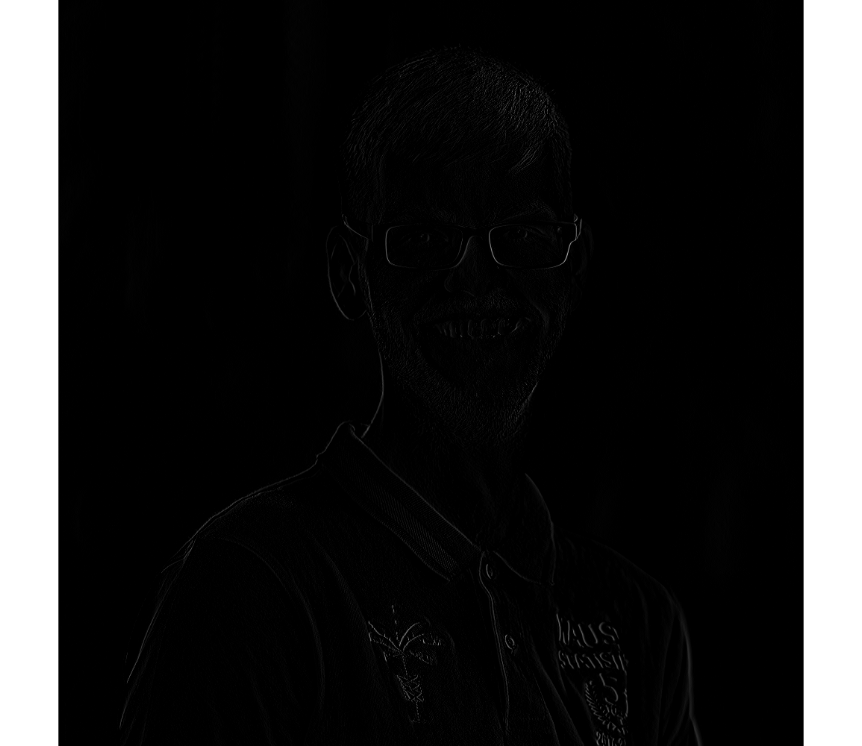
\includegraphics[width=0.5\linewidth]{Images/conv4.png}
\end{figure}
Now we're picking up some features!
\end{frame}

\begin{frame}{Image convolutions}
Third kernel? Sharpens.

\begin{minipage}{0.65\linewidth}
$ * \left[\begin{pmatrix}
0 & 0 & 0 & 0 &0 \\
0 & 0 & 0 & 0 &0 \\
0 & 0 & 2 & 0 &0 \\
0 & 0 & 0 & 0 &0 \\
0 & 0 & 0 & 0 &0 \\
\end{pmatrix}-\frac{1}{25}\begin{pmatrix}
1 & 1 & 1 & 1 &1 \\
1 & 1 & 1 & 1 &1 \\
1 & 1 & 1 & 1 &1 \\
1 & 1 & 1 & 1 &1 \\
1 & 1 & 1 & 1 &1 \\
\end{pmatrix}\right] =$
\end{minipage}
\begin{minipage}{0.32\linewidth}
\begin{figure}
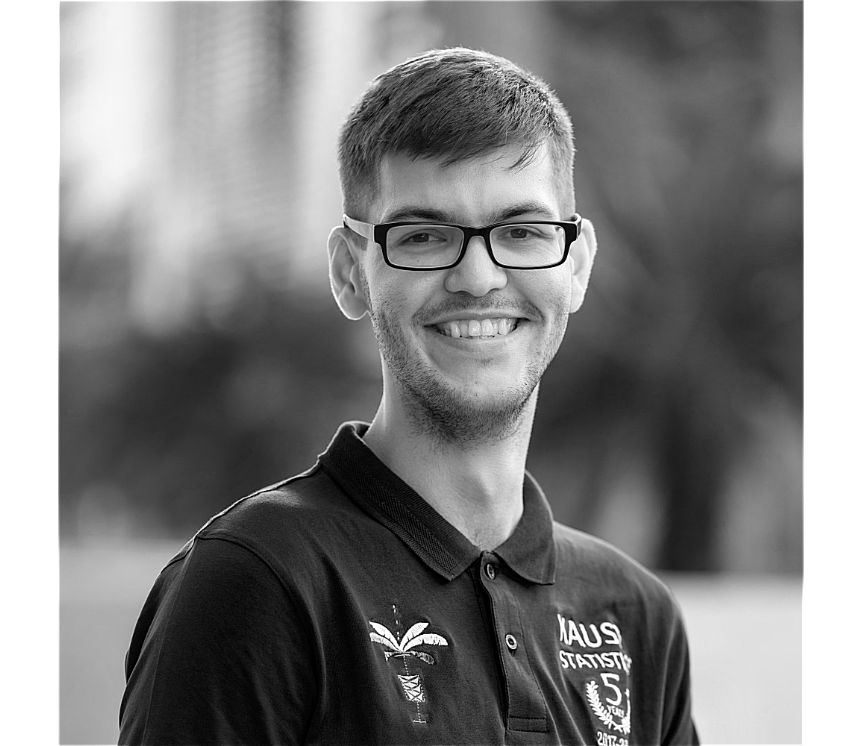
\includegraphics[width=\linewidth]{Images/conv5.png}
\end{figure}
\end{minipage}
\end{frame}

\begin{frame}{Image convolutions}
$x$-axis edge detection

\begin{minipage}{0.32\linewidth}
\begin{figure}
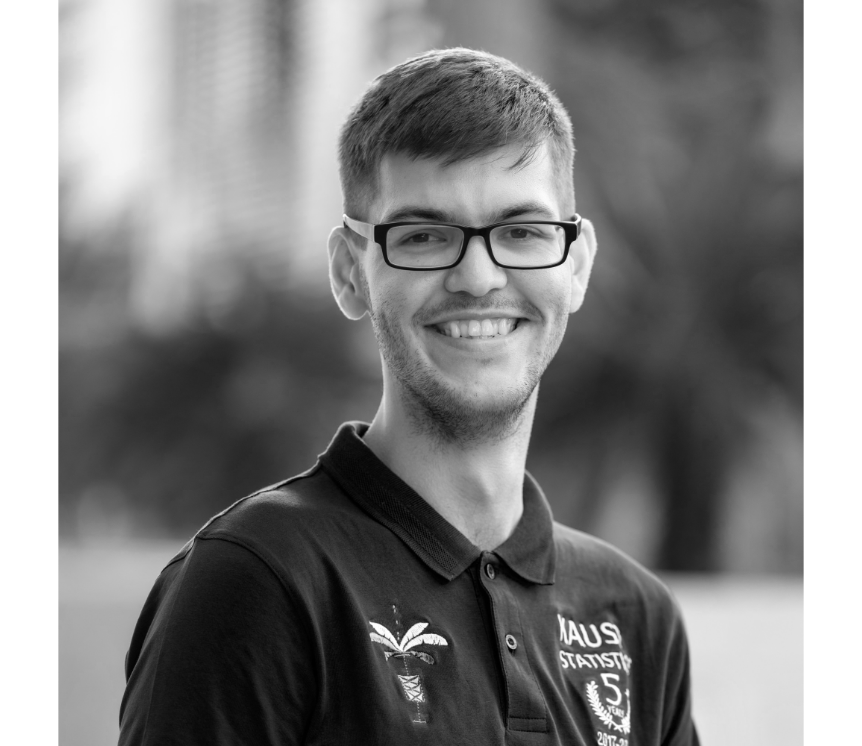
\includegraphics[width=\linewidth]{Images/conv1.png}
\end{figure}

\end{minipage}
\begin{minipage}{0.32\linewidth}
$ * \begin{pmatrix}
-1& 0 & 1 \\
-2& 0 & 2 \\
-1& 0 & 1 \\
\end{pmatrix} =$
\end{minipage}
\begin{minipage}{0.32\linewidth}
\begin{figure}
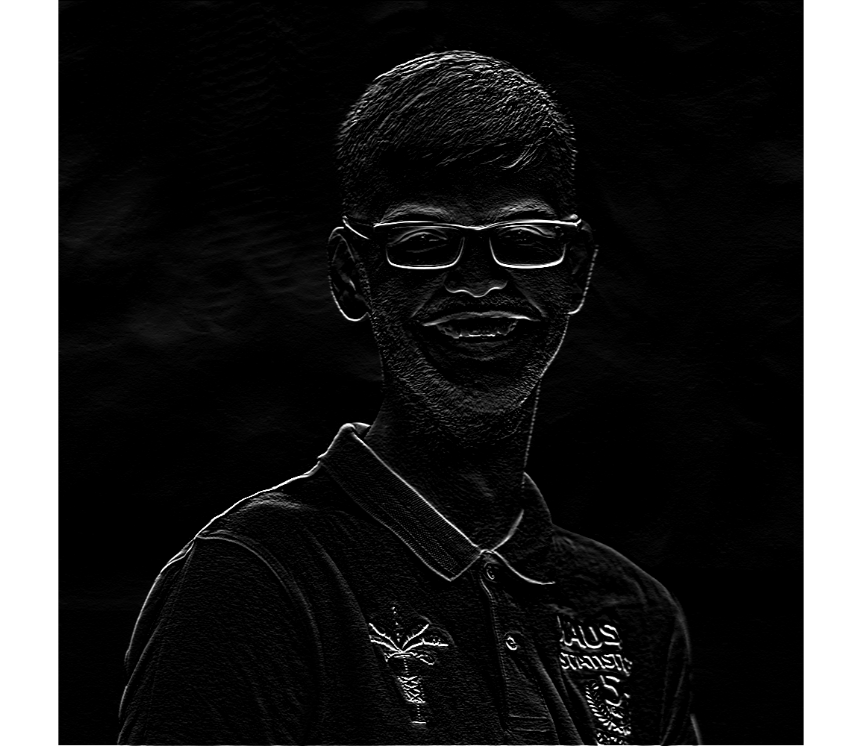
\includegraphics[width=\linewidth]{Images/conv6.png}
\end{figure}
\end{minipage}
\end{frame}

\begin{frame}{Image convolutions}
$y$-axis edge detection

\begin{minipage}{0.32\linewidth}
\begin{figure}
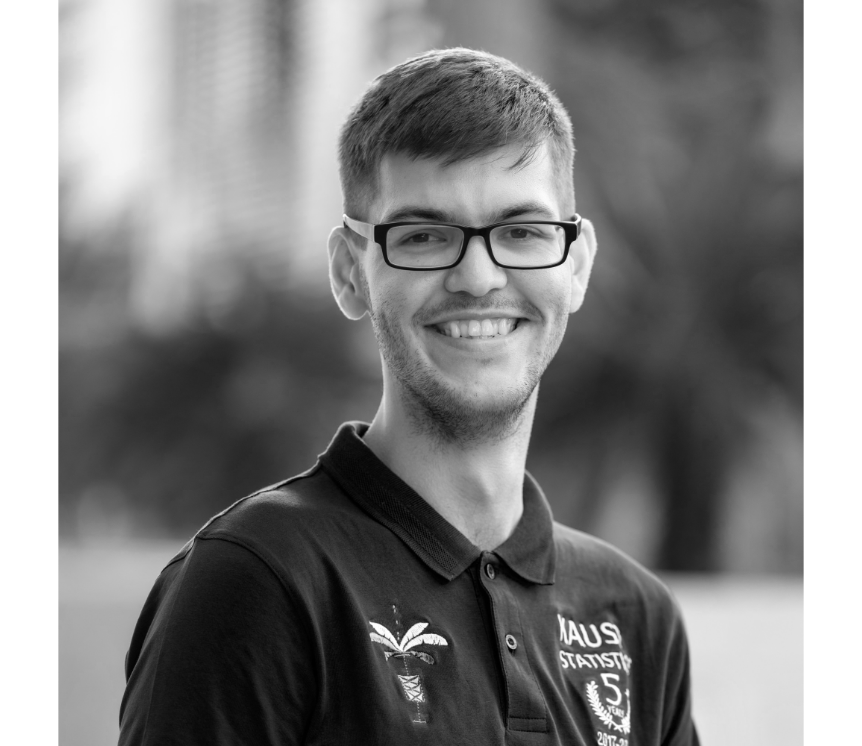
\includegraphics[width=\linewidth]{Images/conv1.png}
\end{figure}

\end{minipage}
\begin{minipage}{0.32\linewidth}
$ * \begin{pmatrix}
-1& -2 & -1 \\
0& 0 & 0 \\
1& 2 & 1 \\
\end{pmatrix} =$
\end{minipage}
\begin{minipage}{0.32\linewidth}
\begin{figure}
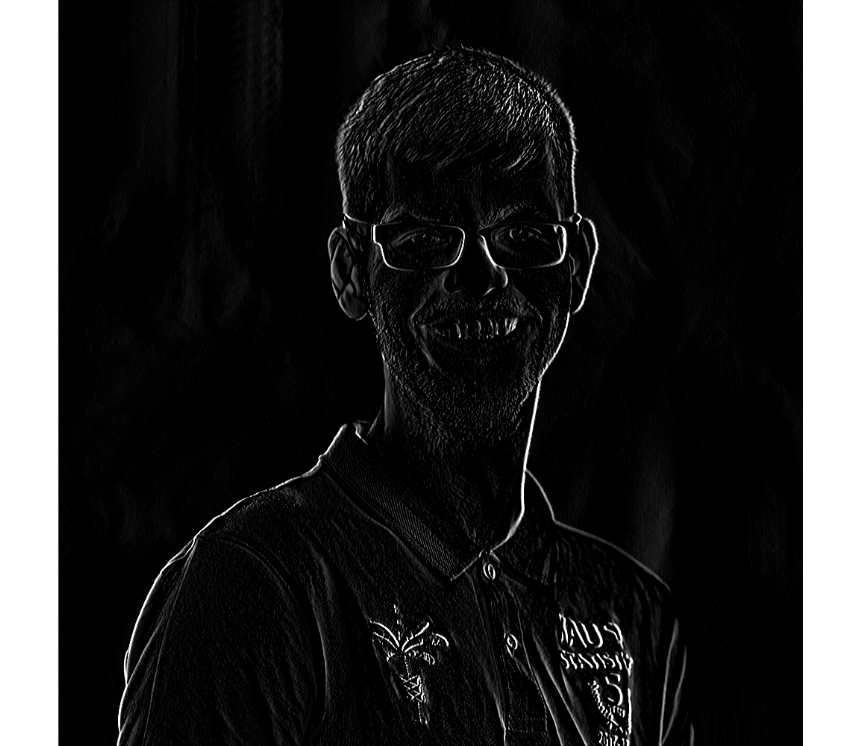
\includegraphics[width=\linewidth]{Images/conv7.png}
\end{figure}
\end{minipage}
\end{frame}

\begin{frame}{Image convolutions}
Laplacian kernel - all edge detection

\begin{minipage}{0.32\linewidth}
\begin{figure}
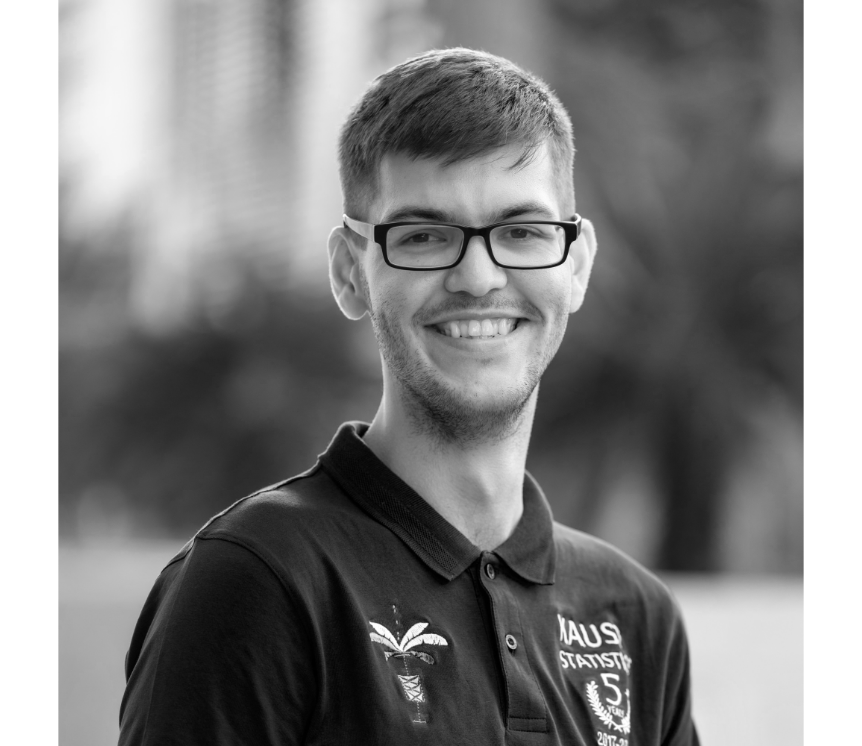
\includegraphics[width=\linewidth]{Images/conv1.png}
\end{figure}

\end{minipage}
\begin{minipage}{0.32\linewidth}
$ * \begin{pmatrix}
0 & -1 & 0 \\
-1 & 4 & -1\\
0& -1 & 0\\
\end{pmatrix} =$
\end{minipage}
\begin{minipage}{0.32\linewidth}
\begin{figure}
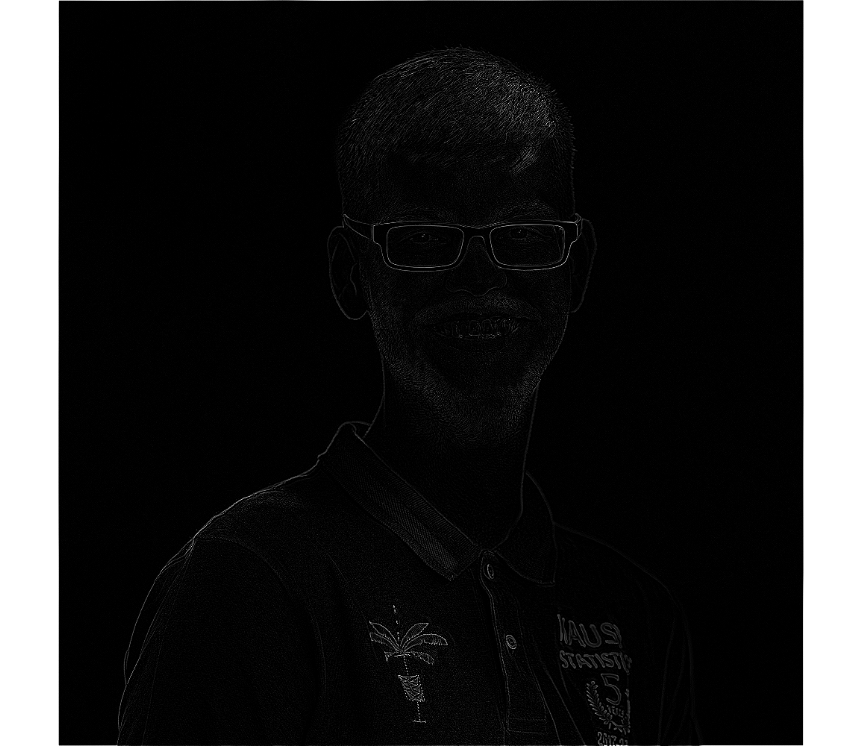
\includegraphics[width=\linewidth]{Images/conv8.png}
\end{figure}
\end{minipage}
\end{frame}

\begin{frame}{Image convolutions}
Random kernel - all weights drawn from Unif(-2,2)

\begin{minipage}{0.24\linewidth}
\begin{figure}
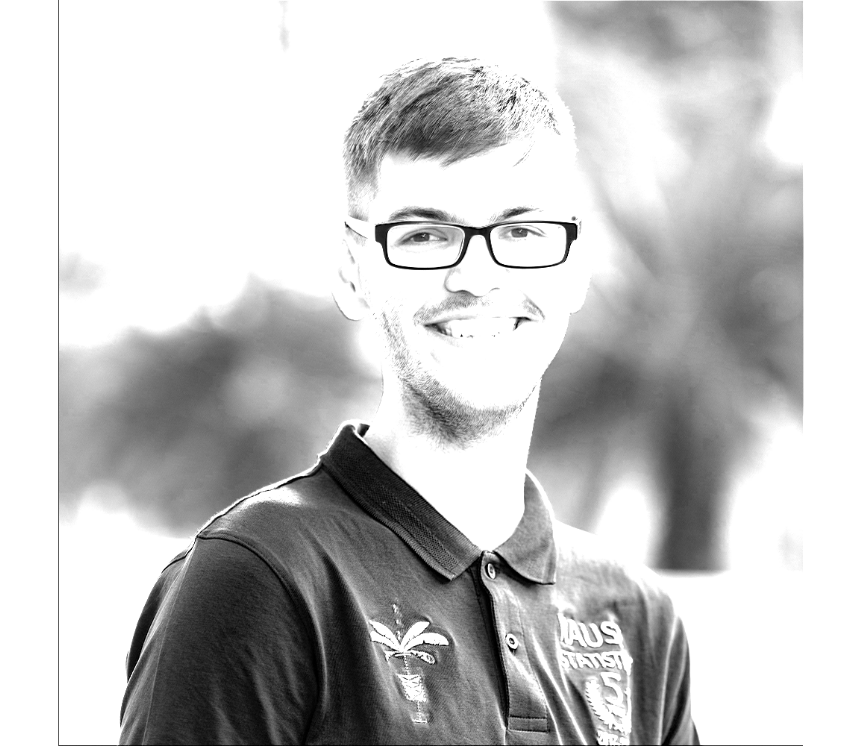
\includegraphics[width=\linewidth]{Images/conv11.png}
\end{figure}

\end{minipage}
\begin{minipage}{0.24\linewidth}
\begin{figure}
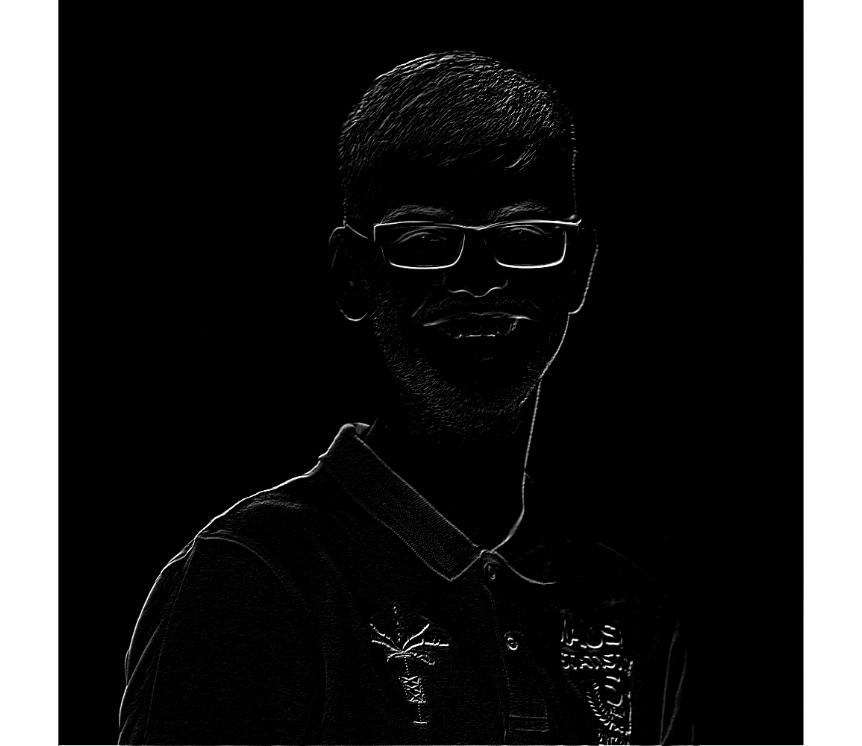
\includegraphics[width=\linewidth]{Images/conv12.png}
\end{figure}

\end{minipage}
\begin{minipage}{0.24\linewidth}
\begin{figure}
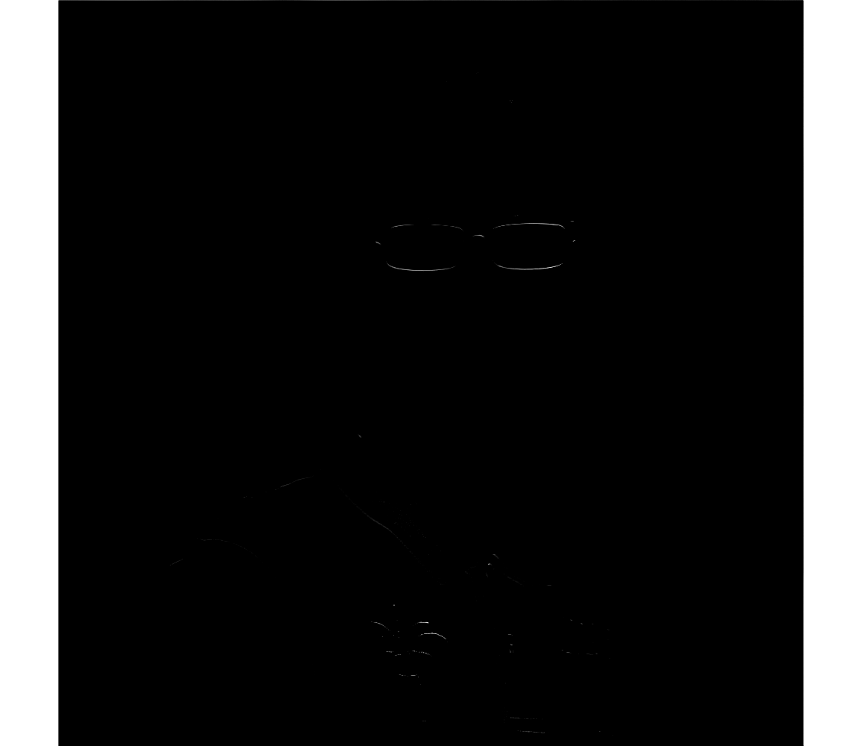
\includegraphics[width=\linewidth]{Images/conv13.png}
\end{figure}

\end{minipage}
\begin{minipage}{0.24\linewidth}
\begin{figure}
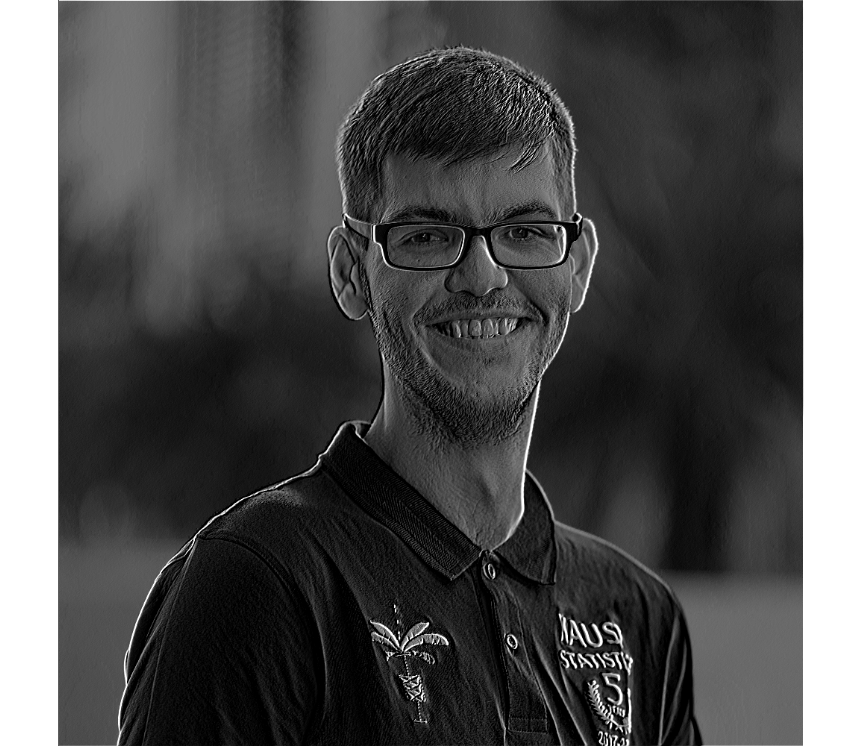
\includegraphics[width=\linewidth]{Images/conv14.png}
\end{figure}

\end{minipage}
Lots of different features extracted. Ideally, we want an algorithm that can learn the kernel weights, rather than pre-specifying them. We call every convolved image in a CNN a \textbf{feature map}.
\end{frame}

\begin{frame}{Image convolutions}
\textbf{Tensors}: In practice, input (images) are often tensors, so that there is a multivariate value at each spatial location (pixel). For example, in \textbf{RGB} color images, there are three values (associated with red, green and blue intensities) that define the overall colour of a pixel color.\\
If the input is RGB, a CNN considers a tensor convolution where the kernel averages  over location and the variables (referred to as ''\textbf{channels}'').
\end{frame}


\begin{frame}{Convolution layers\footnote{Copyright belongs to \url{https://machinelearningmastery.com/convolutional-layers-for-deep-learning-neural-networks/}}}
A \textbf{convolution layer} acts on an image, not a vector of inputs. The image can be 1D (e.g., text), 2D or 3D (e.g., a video or 3D model)
\begin{minipage}{0.49\linewidth}
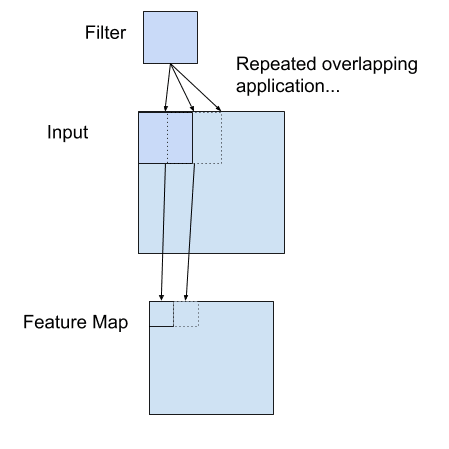
\includegraphics[width=\textwidth]{Images/cfilter.png}
\end{minipage}
\begin{minipage}{0.49\linewidth}
\begin{itemize}
\item A convolution filter/kernel of a certain dimension is passed over the image
\item The filter starts in a corner of the image. A convolution is performed, and then the filter moves one horizontal ``stride''. Once it reaches the edge, it moves one vertical stride down. 
\end{itemize}
\end{minipage}
\end{frame}
\begin{frame}{Convolution layers\footnote{Copyright belongs to \url{https://machinelearningmastery.com/convolutional-layers-for-deep-learning-neural-networks/}}}
\begin{minipage}{0.39\linewidth}
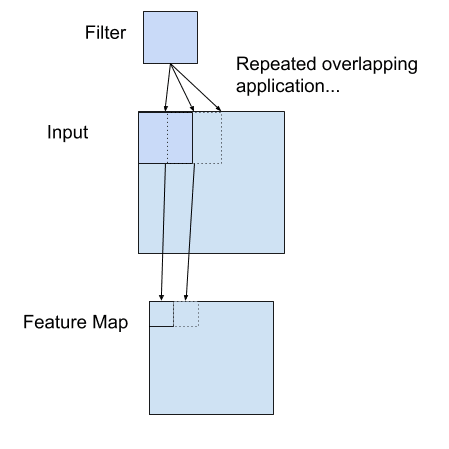
\includegraphics[width=\textwidth]{Images/cfilter.png}
\end{minipage}
\begin{minipage}{0.59\linewidth}
\begin{itemize}
\item After the filter has passed over the entire image, a \textbf{feature map} will be produced. The dimension of the feature map will be determined by the filter dimension and the strides
\item An image can have multiple ``channels'', i.e., different colours, inputs, each with its own filter
\item The feature maps for the different channels are added, a bias is introduced and then $a$ is applied 
\item A layer can have \textbf{multiple filters}, similar to nodes in a densely-connected network
\end{itemize}
\end{minipage}
\end{frame}

\begin{frame}{CNNs}
\begin{itemize}
\item One of the strengths of CNNs is that it learns kernel weights, but \textbf{reduces the parameter space} by assuming that there is only one set of weights for each convolution. This ability to share weights leads to a huge dimension reduction in the parameter space (compared to a DNN).
\item Then CNN considers a convolution of the image with unknown weights that are learned.
\item Then the convolution step is followed by a \textbf{pooling layer} (or, ``subsampling'' or ``downsampling''), which further reduces the dimension.
\end{itemize}
\end{frame}

\begin{frame}{Pooling}
A limitation of convolutional layers is that they \textbf{record the precise position of features in the input}. This means that small movements in the position of the feature in the input image will result in a different feature map. This can happen when applying cropping, rotation, shifting, and other minor changes to the input image.
\begin{itemize}
\item We can make a CNN more \textbf{robust to image translations} by using downsampling. This can be achieved by varying the stride of the convolution kernel or (more commonly) via pooling.
\item The pooling layer considers a small rectangular block from the convolutional step and subsamples it in some way to produce a single output. The most common type of pooling is \textbf{max-pooling}, where we just sample the maximum value in a block (from a $2\times 2$ window with stride 2).
\item Note that this is also a form of dimension reduction.
\item Implemented with $\texttt{layer\_max\_pooling\_2d}$.
\end{itemize}
\end{frame}

\begin{frame}{Max-pooling: example}
With Laplacian kernel - all edge detection

\begin{minipage}{0.32\linewidth}
\begin{figure}
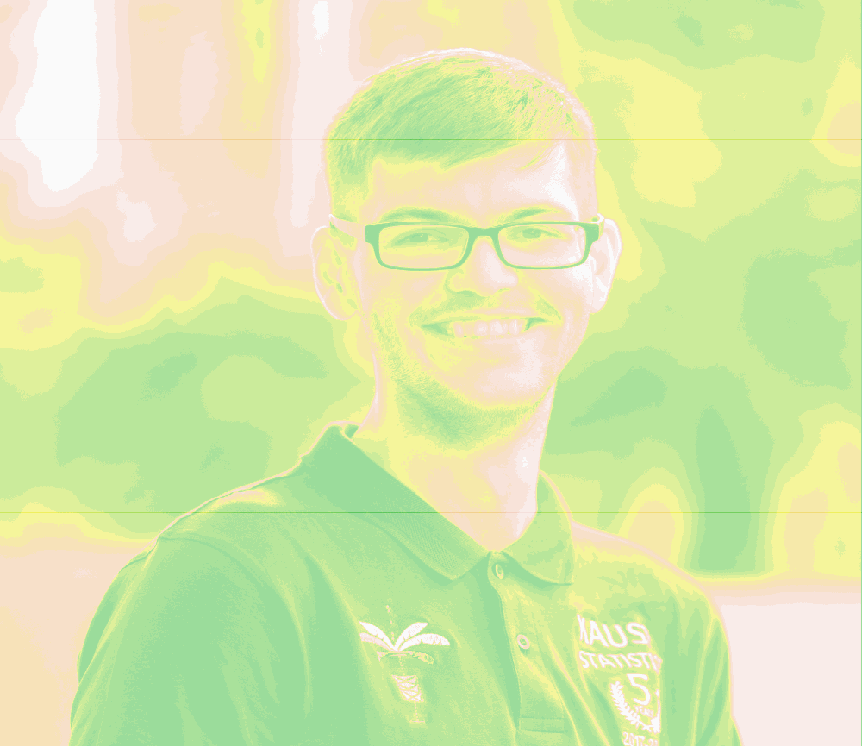
\includegraphics[width=\linewidth]{Images/conv15.png}
\end{figure}

\end{minipage}
\begin{minipage}{0.32\linewidth}
$ * \begin{pmatrix}
0 & -1 & 0 \\
-1 & 4 & -1\\
0& -1 & 0\\
\end{pmatrix} =$
\end{minipage}
\begin{minipage}{0.32\linewidth}
\begin{figure}
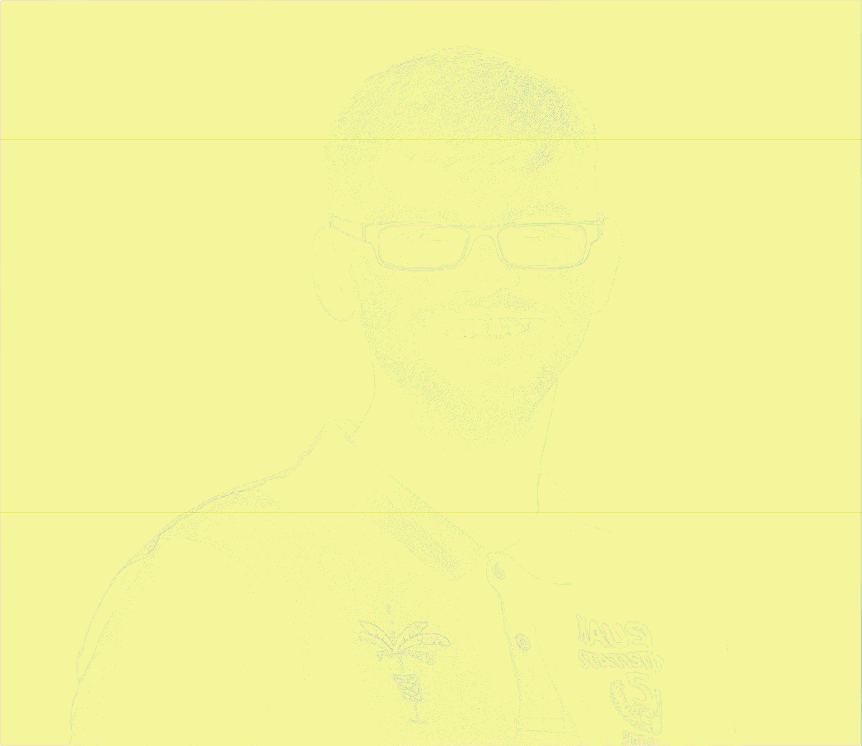
\includegraphics[width=\linewidth]{Images/conv16.png}
\end{figure}
\end{minipage}
\end{frame}
\begin{frame}{Max-pooling: example}

\begin{minipage}{0.32\linewidth}
\begin{figure}
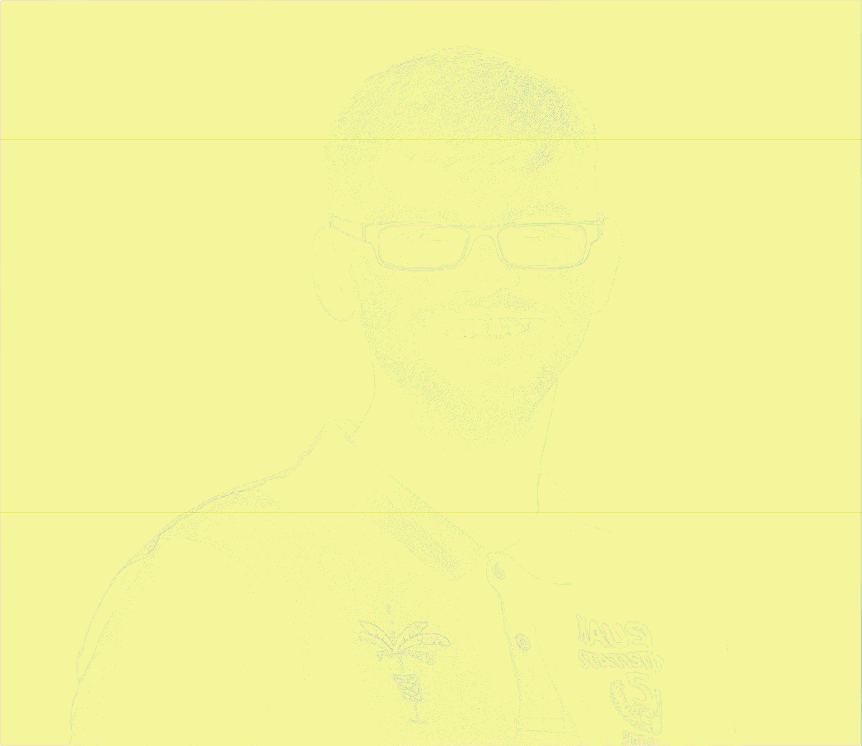
\includegraphics[width=\linewidth]{Images/conv16.png}
\end{figure}

\end{minipage}
\begin{minipage}{0.32\linewidth}
$*$ $2 \times 2$ max-pool
\end{minipage}
\begin{minipage}{0.32\linewidth}
\begin{figure}
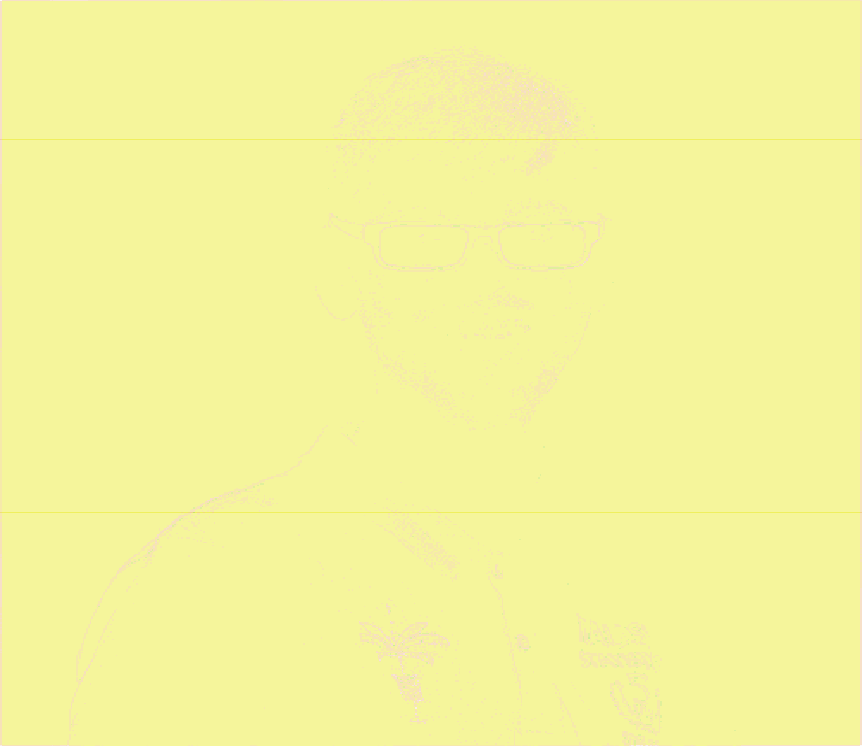
\includegraphics[width=\linewidth]{Images/conv17.png}
\end{figure}
\end{minipage}
\end{frame}
\begin{frame}{Max-pooling: example}

\begin{minipage}{0.32\linewidth}
\begin{figure}
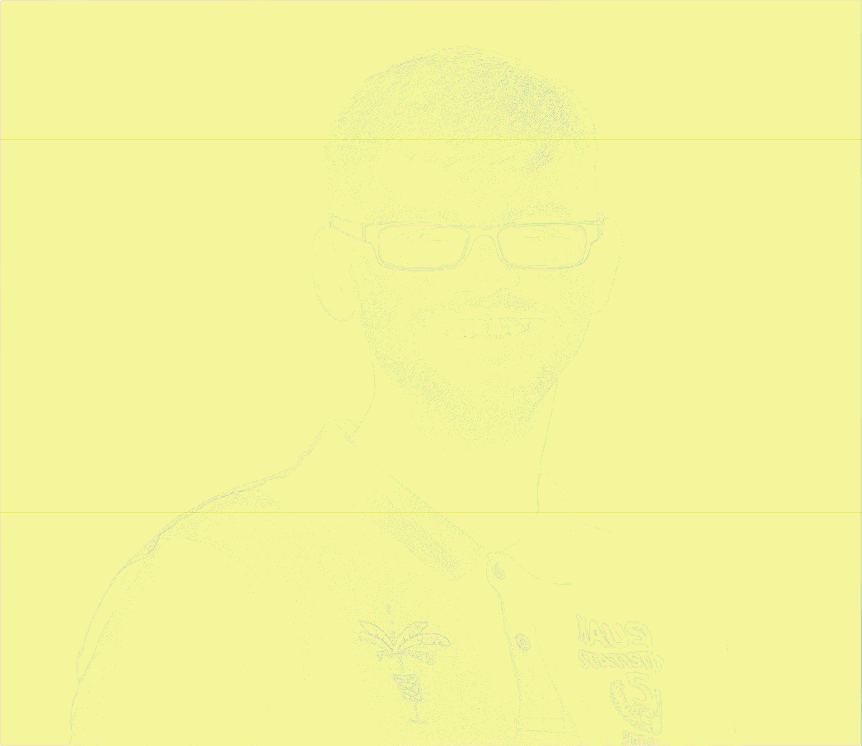
\includegraphics[width=\linewidth]{Images/conv16.png}
\end{figure}

\end{minipage}
\begin{minipage}{0.32\linewidth}
$ *$ $5 \times 5$ max-pool
\end{minipage}
\begin{minipage}{0.32\linewidth}
\begin{figure}
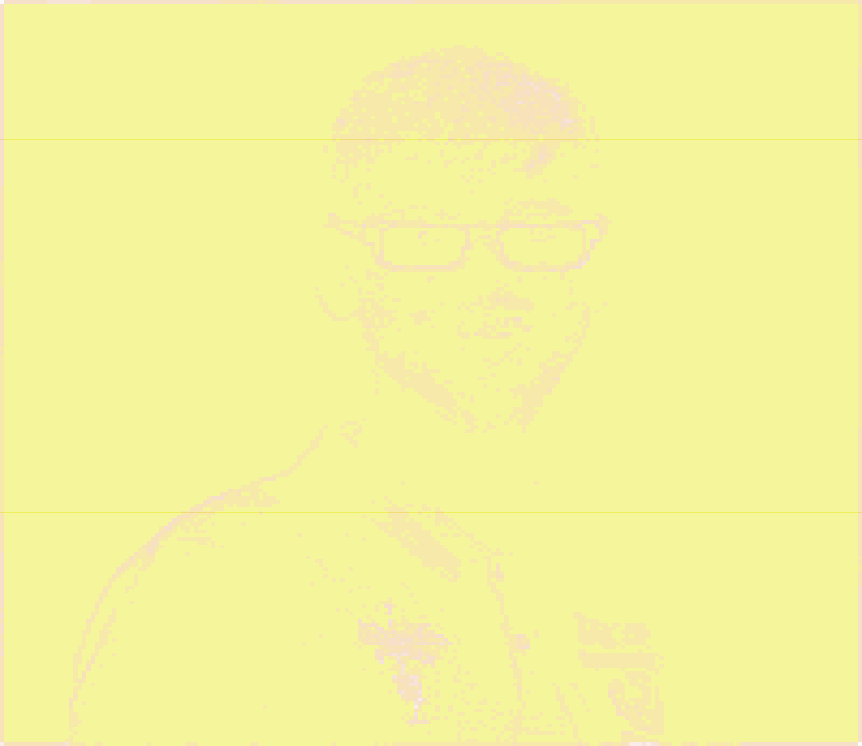
\includegraphics[width=\linewidth]{Images/conv18.png}
\end{figure}
\end{minipage}
\vfill
Note that the same hidden feature map is produced even if the original image is shifted up to five pixels in any direction.
\end{frame}

\begin{frame}{CNN architecture}
The general structure of a CNN has alternating convolution layers
and pooling layers, with the image/feature map dimension decreasing monotonically; the last layer is \textbf{flattened
and fully connected}, as with MLPs.
\begin{figure}
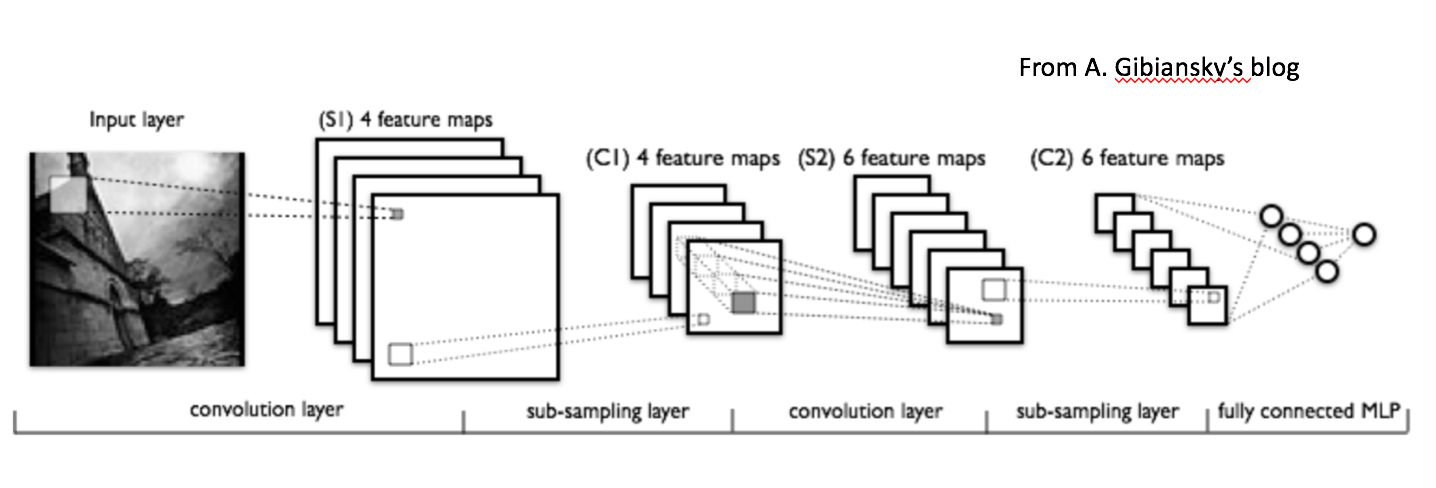
\includegraphics[width=0.8\linewidth]{Images/CNNstructure.png}
\end{figure}
\begin{itemize}
\item For each convolution, multiple feature maps are created using different filters with different weights

\item Bias is added to the convolved images and then they go through an activation function - typically ReLU
\end{itemize}
\end{frame}

\begin{frame}{CNN architecture}
Original LeCun CNN for MNIST handwriting:
\begin{figure}
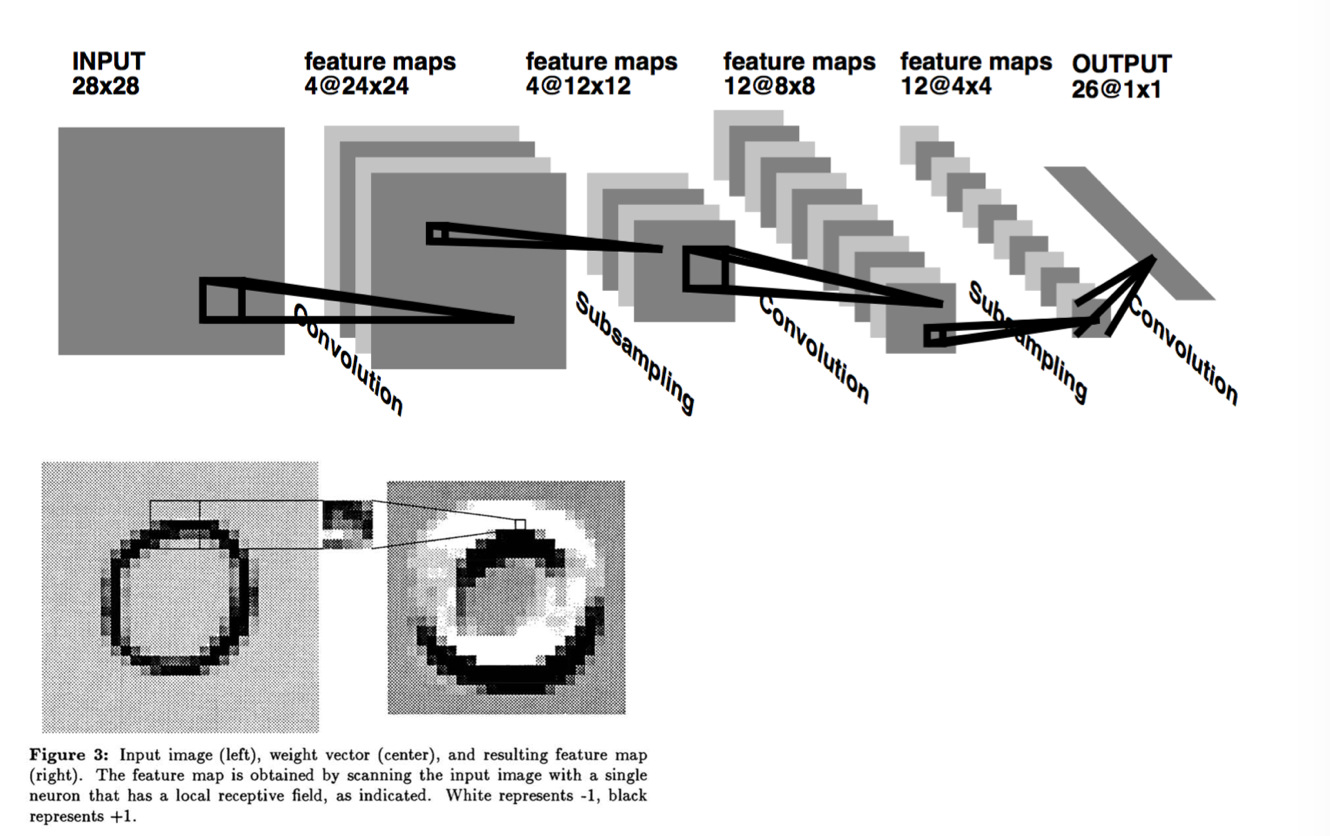
\includegraphics[width=0.9\linewidth]{Images/CNNorig.png}
\end{figure}
\end{frame}

\begin{frame}{CNN implementation}
\begin{itemize}
\item The critical stage of the CNN that requires training is the convolution step; the pooling layers are typically pre-specified and are not learned).
\item Parameters for convolutions for any given filter are the same for the entire feature map. This parameter sharing is important as it allows the presence of a shape in any part of the feature map to be processed in the same way, regardless of its particular spatial location; i.e., it is \textbf{translation invariant}.
\item Each feature in the final convolution layer is connected to each hidden state in the first fully connected layer. This layer works exactly like the layers in a deep FNN. Most of the parameters in a CNN occur in these final layers (e.g., if each of two fully connected layers has 4096 hidden units, then the connections between them will have 16 million weights!).
\end{itemize}
\end{frame}

\begin{frame}{CNN implementation}
\begin{itemize}
\item As before, we use \textbf{backpropagation} to train the CNN.
\item The points about \textbf{regularisation} and \textbf{over-fitting} still apply!
\item Two extra considerations:
\begin{itemize}
\item Images can be padded to keep the dimension the same; useful if you want to output an image, rather than a vector $\hat{\mathbf{y}}$!
\item \textbf{Data augmentation}; unlike FNNs, we can add extra samples for training through random transformations of images!
\end{itemize}
\end{itemize}
\end{frame}
\begin{frame}{Data augmentation}
\begin{figure}
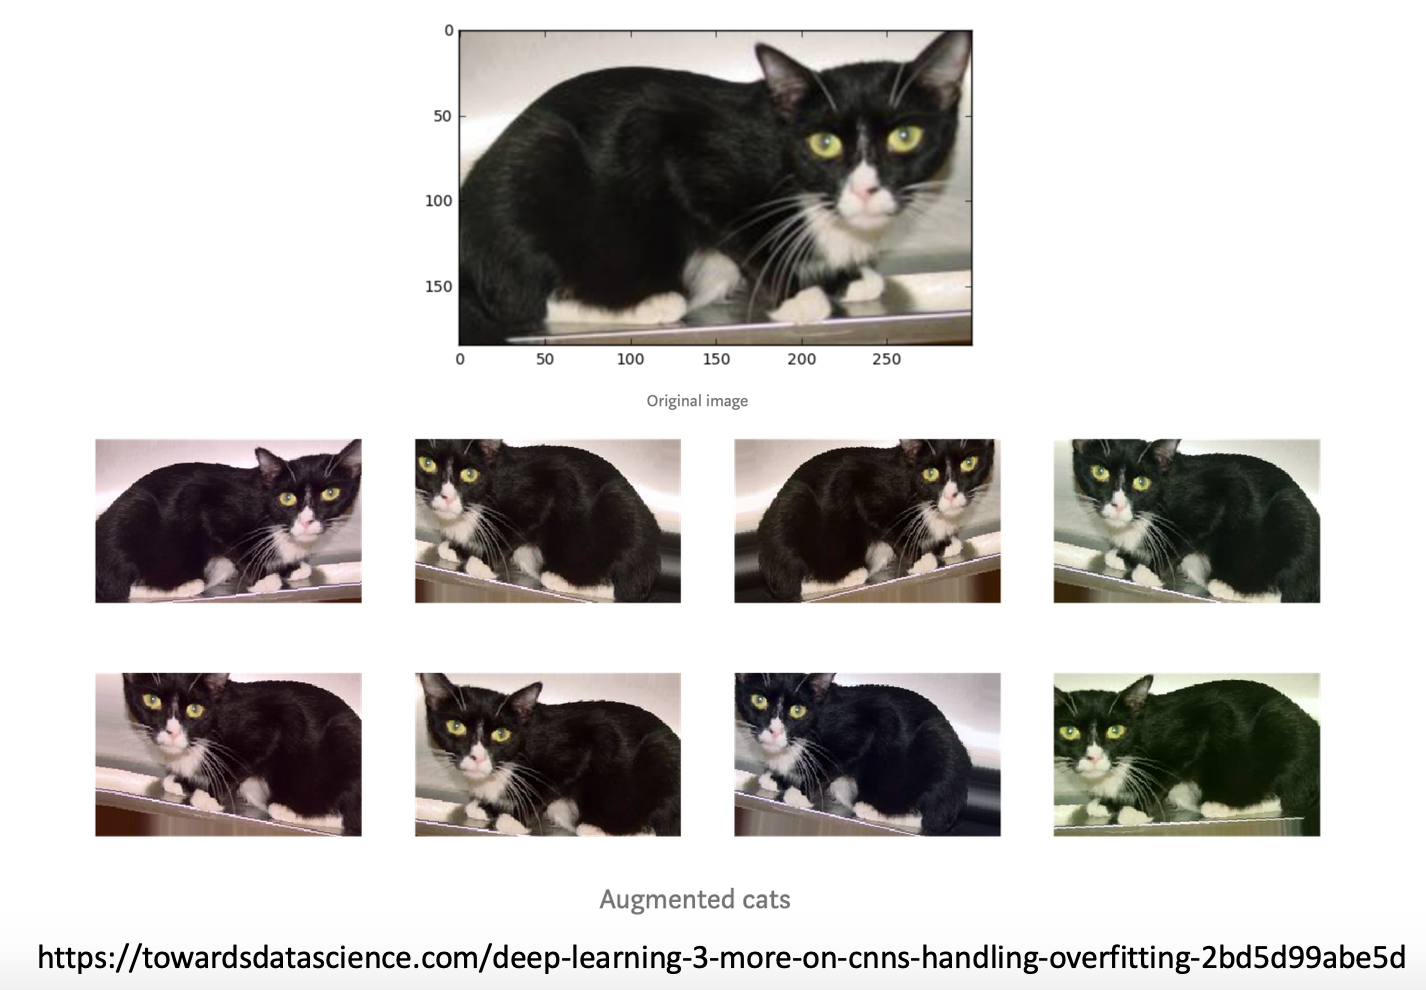
\includegraphics[width=0.9\linewidth]{Images/cat.png}
\end{figure}
\end{frame}
\begin{frame}
\begin{center}
\Huge Recurrent neural networks
\end{center}
\end{frame}
\section{Recurrent neural networks}
\begin{frame}{Recurrent neural networks}
The types of FFNNs that we have covered thus far do not explicitly account for \textbf{sequential/temporal dependence} between inputs and outputs. \\
This gives them limited capacity for solving tasks which depend on the sequential nature of an input, e.g.,
\begin{itemize}
\item Document and time-series classification
\item Speech recognition
\item Sequence-to-sequence learning (language translation)
\item Sentiment analysis
\item Forecasting
\end{itemize}

\end{frame}
\begin{frame}{Recurrent neural networks}
Recurrent Neural Networks (RNNs) were originally developed in the 1980s as feedback models for sequence data. In recent years, they have become one of the \textbf{most used and successful deep learning methods}, particularly for language processing applications.\\
These models are closely related to multivariate state-space models for \textbf{dynamical systems}, as one might see in time series, econometrics, or spatio-temporal statistics.

\end{frame}
\begin{frame}{Dynamical systems}
A classical dynamical system can be written by

$$
\mathbf{s}_{t}=f\left(\mathbf{s}_{t-1} ; \boldsymbol{\theta}\right),
$$

where $\mathbf{s}_{t}$ represents the state of the system at time $t$. This is considered ''recurrent'' because the state at time $t$ refers back to the state at time $t-1$. We can ``unfold'' this into

$$
\mathbf{s}_{t}=f\left(\mathbf{s}_{t-1} ; \boldsymbol{\theta}\right)=f\left(f\left(\mathbf{s}_{t-2} ; \boldsymbol{\theta}\right) ; \boldsymbol{\theta}\right)=f\left(f\left(f\left(\mathbf{s}_{t-3} ; \boldsymbol{\theta}\right) ; \boldsymbol{\theta}\right) ; \boldsymbol{\theta}\right) \ldots
$$

Note, the parameters $\theta$ are shared across all states. 
\end{frame}




\begin{frame}{RNNs\footnote{Copyright belongs to \url{https://www.ibm.com/cloud/learn/recurrent-neural-networks}}}
A recurrent layer takes in as input a sequence of vectors/images. Let's say that the input is the sequence of vectors $\{\mathbf{x}_t:t=1,\dots,T\}$ where $\mathbf{x}_t\in\mathbb{R}^d$ for all $t$.

\begin{figure}
\centering
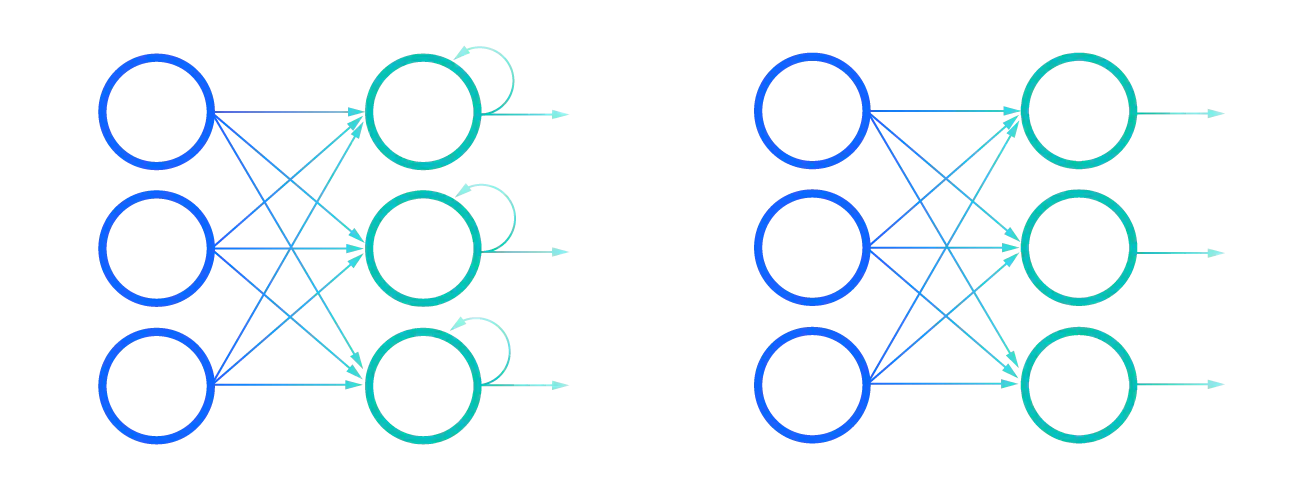
\includegraphics[width=0.7\textwidth]{Images/rnn.png}
\end{figure}
Once an input enters the layer, it becomes stuck in a \textbf{recurrence loop} - the output from the computation using the first input vector $\mathbf{x}_1$ becomes an input for the computation on $\mathbf{x}_2$ (and so on...).
\end{frame}

\begin{frame}{RNNs}
In an RNN, as with a traditional state space model, the states are typically considered ``hidden'' (we denote these hidden states $\mathbf{h}_{t}$) and add external inputs $\mathbf{x}_{t}$:
$$
\mathbf{h}_{t}=f\left(\textcolor{blue}{\mathbf{h}_{t-1}}, \mathbf{x}_{t} ; \boldsymbol{\theta}\right)
$$
So, sequences are processed by iterating through the sequence elements and maintaining a state containing information relative to what it has seen so far via an internal feedback loop. The following image shows how this is unfolded into a computational graph structure:
\begin{figure}
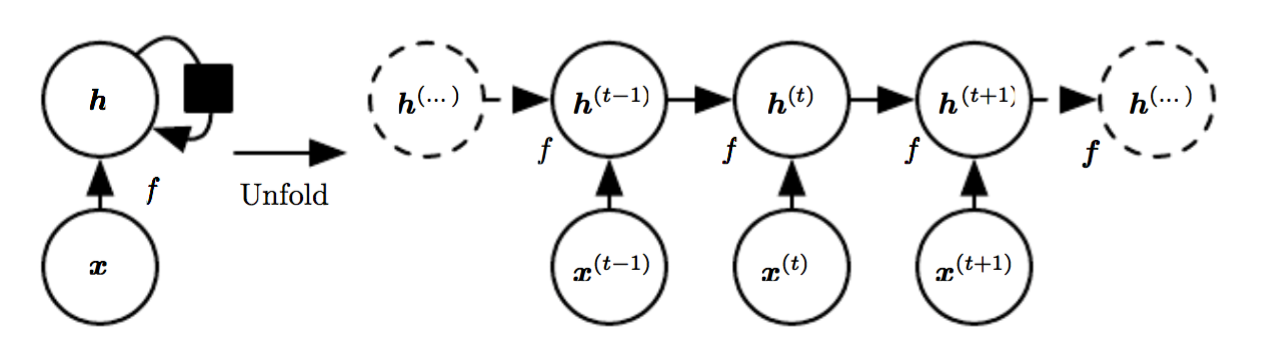
\includegraphics[width=0.86\linewidth]{Images/RNN1.png}
\end{figure}
\centering \copyright C. K. Wikle and D. Pagendam 
\end{frame}
\begin{frame}{RNNs}
A single-layered in a basic ("vanilla") RNN can be written as

$$
\begin{gathered}
\hat{\mathbf{y}}_{t}=g_{o}\left(\mathbf{o}_{t}\right) \\
\mathbf{o}_{t}=\mathbf{W}_{h \hat{y}} \mathbf{h}_{t} \\
\mathbf{h}_{t}=g_{h}\left(\mathbf{W}_{h h} \mathbf{h}_{t-1}+\mathbf{W}_{x h} \mathbf{x}_{t}\right)
\end{gathered}
$$

for activation functions $g_{o}(\cdot), g_{h}(\cdot)$, and weight matrices $\mathbf{W}_{h \hat{y}}$, $\mathbf{W}_{h h}$, and $\mathbf{W}_{x h}$ (typically, these contain bias terms as well).\\
Note that \textbf{equivalence with a FFNN} is given by setting all elements of $\mathbf{W}_{h h}$ to zero!

\end{frame}
 
\begin{frame}{Some points...}
\begin{itemize}
\item Weights in an RNN layer are estimated using ``\textbf{backpropogation through time}'' - a slight extension of backpropogation which accounts for the shared parameters across time
\item RNN layers can be stacked on top of each other - we can choose for $\texttt{Keras}$ to output the entire series of vectors in a hidden layer $(\mathbf{h}_t)^T_{t=1}$ or just one vector, e.g.,  $\mathbf{h}_T$
\item These simple layers can be implemented using $\texttt{layer\_simple\_rnn}$
\item Input into $\texttt{Keras}$ is a tensor with axes $[n,T,p]$
\end{itemize}
\end{frame}

\begin{frame}{LSTMs}
\begin{itemize}
\item Generally simple RNNs aren't used in practice now due to the so-called vanishing/exploding problem. Diminishing time series dependence leads to exponentially smaller weights for long time series.
\item Not all information from the past needs to be remembered! Some RNNs add ``\textbf{gates}'' that selectively allows information from the past to influence the future state. These gates retain information for later and have their own internal memory.
\item One of the most famous type are \textbf{Long Short-Term Memory} networks\footnote{S. Hochreiter; J. Schmidhuber (1997). ''Long short-term memory''. Neural Computation. 9 (8): 1735–1780.}, implementable by $\texttt{layer\_lstm}$.
\end{itemize}

\end{frame}
\begin{frame}{LSTMs}
Consider the basic one-layered LSTM:

$$
\begin{gathered}
\text { Output: } \quad \mathbf{y}_{t}=g_{o}\left(\mathbf{V h}_{t}\right) \\
\text { Hidden State: } \quad \mathbf{h}_{t}=\tanh \left(\mathbf{c}_{t}\right) \odot \mathbf{o} \\
\text { Internal Memory: } \quad \mathbf{c}_{t}=\mathbf{c}_{t-1} \odot \mathbf{f}+\mathbf{g} \odot \mathbf{i} \\
\text { Candidate Hidden State: } \quad \mathbf{g}=\tanh \left(\mathbf{U}^{g} \mathbf{x}_{t}+\mathbf{W}^{g} \mathbf{h}_{t-1}\right) \\
\text { Output Gate: } \quad \mathbf{o}=g\left(\mathbf{U}^{o} \mathbf{x}_{t}+\mathbf{W}^{o} \mathbf{h}_{t-1}\right) \\
\text { Forget Gate: } \quad \mathbf{f}=g\left(\mathbf{U}^{f} \mathbf{x}_{t}+\mathbf{W}^{f} \mathbf{h}_{t-1}\right) \\
\text { Input Gate: } \quad \mathbf{i}=g\left(\mathbf{U}^{i} \mathbf{x}_{t}+\mathbf{W}^{i} \mathbf{h}_{t-1}\right)
\end{gathered}
$$

where $g(\cdot)$ is a sigmoid function.
\end{frame}

\begin{frame}{LSTMs}
\begin{figure}
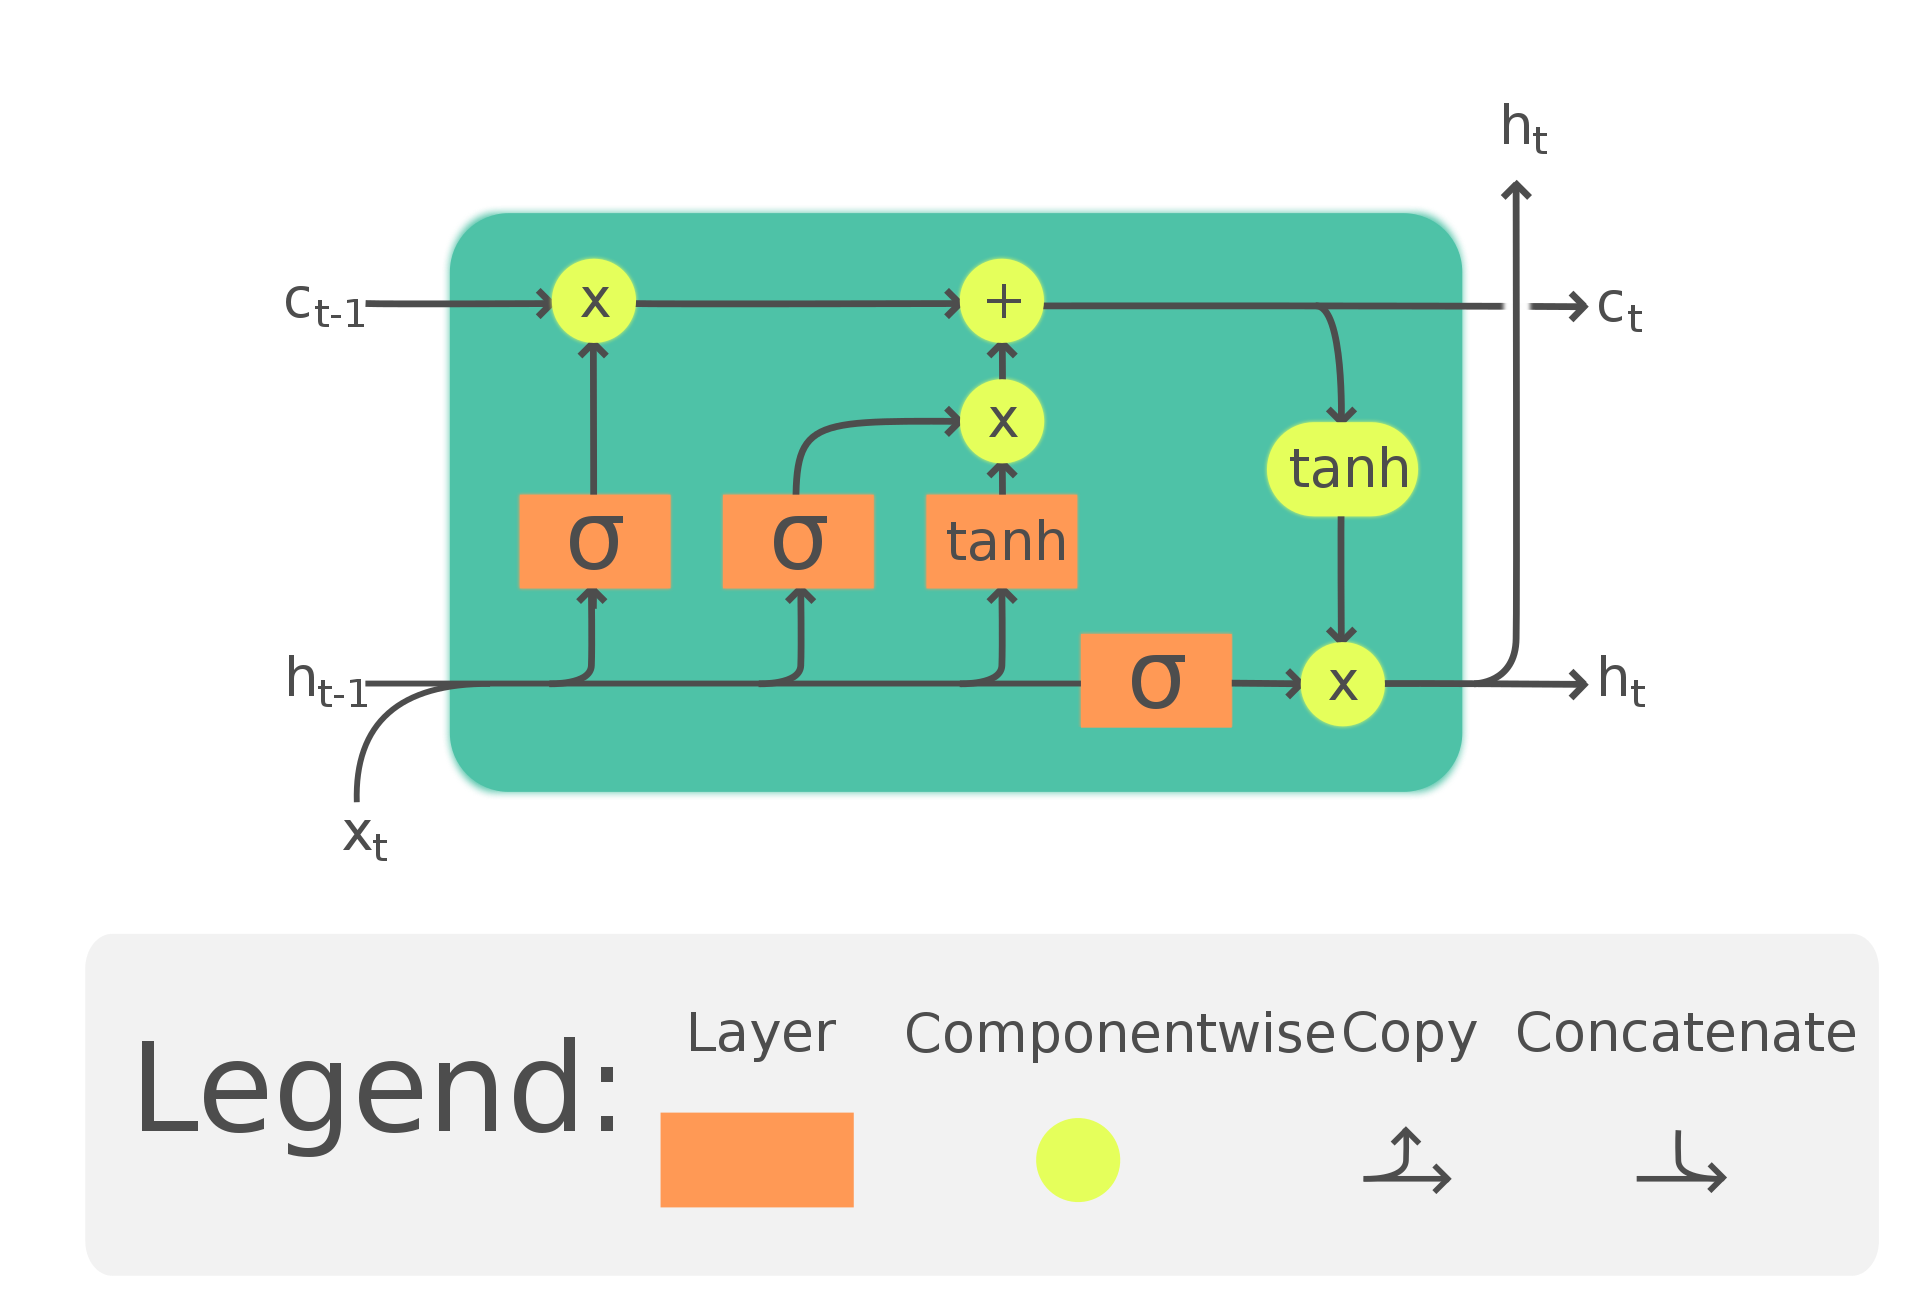
\includegraphics[width=0.5\linewidth]{Images/LSTM_Cell.png}
\end{figure}
\begin{itemize}
\item Forget gates  $\mathbf{f}$ decide what information to \textbf{forget} from the previous memory state.
\item Input gates $\mathbf{i}$ decide which pieces of new information $\mathbf{g}$ to store in the current memory state 
\item Output gates $\mathbf{o}$ control which pieces of information in the current memory state to output. 
\end{itemize}
\end{frame}



\begin{frame}{Final points...}
\begin{itemize}
\item You don't need to really understand the structure for LSTMs; just apply the model!
\item We considered a dense ``vanilla'' recurrent layer. We can have recurrent convolutional layers instead (see e.g., $\texttt{layer\_conv\_lstm\_2d}$), which captures temporal structure within sequences of images
\end{itemize}
\end{frame}

\section{Graph neural networks}
\begin{frame}
\begin{center}
\Huge Graph neural networks
\end{center}
\end{frame}
\begin{frame}{Overview}

\end{frame}

\begin{frame}
\begin{center}
\Huge Thanks for your attention!
\end{center}
\end{frame}
\end{document}
